\documentclass[pdflatex,sn-mathphys-num]{sn-jnl}

% Standard packages compatible with sn-jnl (do not load natbib, geometry, or hyperref manually)
\usepackage{graphicx}
\usepackage{multirow}
\usepackage{amsmath,amssymb,amsfonts}
\usepackage{amsthm}
\usepackage{booktabs}
\usepackage{array}
\usepackage{url}

\raggedbottom

\begin{document}

\title[Edge Vietnamese ALPR Optimization and Robustness Benchmark]{Eliminating Hidden Compute-Bound Bottlenecks and Evaluating Compression Robustness for Edge Vietnamese License Plate Recognition}

%%=============================================================%%
%% Author metadata: replace placeholders with full names/emails
%% Project team roles from Phase 6:
%% Huy (Data Eng), Khanh (Field Data & QA), Hy (Perturbations),
%% Tuan (Metrics), Khoi (Runner & Profiling), Triet (Reporting & Docker)
%%=============================================================%%
\author*[1]{\fnm{Huy} \sur{Ho}}\email{hohuytencent@gmail.com}
\author[1]{\fnm{Khanh} \sur{Nguyen}}
\author[1]{\fnm{Hy} \sur{Le}}
\author[1]{\fnm{Tuan} \sur{Tran}}
\author[1]{\fnm{Khoi} \sur{Pham}}
\author[1]{\fnm{Triet} \sur{Nguyen}}

\affil[1]{\orgdiv{Department of Computer Science and Engineering}, \orgname{Research Group on Embedded Computer Vision}, \orgaddress{\city{Ho Chi Minh City}, \country{Vietnam}}}

\abstract{
Deploying Automatic License Plate Recognition (ALPR) on low-cost edge hardware such as the Raspberry Pi requires balancing memory limits, compute throughput, and accuracy under adverse field conditions. Prior edge surveillance work by Jagtap and Dhawale (2025) demonstrated YOLOv8 pruning and INT8 quantization on Raspberry Pi~4 alongside Tesseract OCR, yet left critical reproducibility gaps---undisclosed datasets, ambiguous OCR metrics, and omission of modern deep OCR compute costs. In this work, we design, optimize, and rigorously benchmark a zero-PyTorch, two-stage Vietnamese ALPR pipeline targeting both single-line car plates and two-line square motorcycle plates. First, migrating YOLOv8 to Pure ONNX Runtime with dynamic \texttt{QUInt8} quantization eliminates PyTorch runtime overhead, reducing deployment container images below 350\,MB, trimming detector RAM initialization by 83.8\% (330.96\,MB to 53.61\,MB), and shrinking model weights by 71.2\%--72.6\% while surviving constrained containers down to 256\,MB RAM. Second, Docker cgroup stress testing reveals a shift from memory-bound to severe OCR compute-bound latency (85\%--95\% of total runtime), traced to RapidOCR's default \texttt{limit\_side\_len=736} minimum-side upscaling of small plate crops. By combining $480\times 480$ Pareto resolution scaling, core-matched ONNX intra-op threading, adaptive ROI capping ($H_{\max}=96$\,px), \texttt{limit=320 max}, no-dilation DBNet inference, and disabled angle classification, we accelerate OCR by $5.85\times$ and reduce end-to-end latency on simulated Raspberry Pi~4 from 4,184.24\,ms to 668.74\,ms ($6.26\times$ speedup). Third, to replace non-reproducible weather claims, we establish a transparent two-tier robustness benchmark: 300 clean baseline images (Source~A) expanded into 9,000 synthetic images across 10 perturbation scenarios and 3 severity levels with verified bounding-box lineage, paired with 60 real-world challenging images (Source~B). Evaluating 3,000 corrupted samples per model shows that INT8 compression preserves environmental robustness nearly identically to FP32 ($\Delta\text{mAP@50} = -0.09$\,pp, $\Delta\text{EM} = -0.47$\,pp), while pinpointing early deep OCR collapse under motion blur, partial occlusion, and two-line slanted motorcycle plates as the primary frontier for future edge ALPR research.
}

\keywords{Edge ALPR, YOLOv8 Quantization, ONNX Runtime, Raspberry Pi, Deep OCR Over-Processing, Robustness Benchmark}

\maketitle

\section{Introduction}\label{sec:intro}

Automated vehicle access control at residential compounds, industrial campuses, and toll gates in Vietnam relies heavily on Automatic License Plate Recognition (ALPR). Unlike regions dominated by uniform single-row plates, Vietnamese urban traffic comprises over 70\% motorcycles carrying compact two-line square plates alongside single-line and square car plates. Deploying reliable two-stage ALPR---first localizing the plate region and then reading alphanumeric sequences---on inexpensive single-board computers such as the Raspberry Pi~4, 3, or 2 remains challenging due to tight memory ceilings (512\,MB--2\,GB RAM) and modest ARM CPU compute budgets.

A recent study by Jagtap and Dhawale~\cite{jagtap2025yolo} (hereafter \emph{Paper~23}) investigated YOLOv8-based helmet and number plate detection on Raspberry Pi~4 using L1 weight pruning, dynamic INT8 quantization, ONNX Runtime, and Tesseract OCR~5.0~\cite{smith2007tesseract}. While establishing YOLOv8 as a strong detector baseline, reproducing and extending Paper~23 for Vietnamese edge ALPR exposes five concrete technical and methodological gaps:
\begin{enumerate}
    \item \textbf{Domain mismatch of classical OCR:} Paper~23 relies on Tesseract~5.0 over Indian single-line plates without releasing OCR code or line-ordering heuristics. Classical thresholding and Tesseract frequently scramble character order across Vietnamese two-line motorcycle plates.
    \item \textbf{Hidden OCR compute bottlenecks under modern deep OCR:} Replacing Tesseract with modern lightweight deep OCR (such as RapidOCR/PP-OCR~\cite{liao2020real,li2022ppocrv3}) resolves Vietnamese character layout accuracy, yet immediately shifts execution from memory-bound to severely compute-bound on ARM CPUs---an interaction left unmeasured when Paper~23 reports $<200$\,ms total latency alongside a 32\,ms detector time.
    \item \textbf{Unexplored input scaling and SIMD thread contention:} Fixing detector inputs at $640\times 640$ ignores quadratic matrix scaling $\mathcal{O}(W\times H)$ and thread-oversubscription penalties across 1--4 core ARM processors.
    \item \textbf{Black-box dataset opacity:} Paper~23 describes $\sim$1,000 collected images augmented above 5,000 samples without public access, train/validation/test split ratios, or per-condition sample sizes in its weather breakdown.
    \item \textbf{Ambiguous evaluation metrics:} Paper~23 reports ``OCR Accuracy (\%)'' across weather categories without mathematical definitions separating character accuracy from strict whole-plate Exact Match (EM) or accounting for missed detections.
\end{enumerate}

To close these gaps, this paper presents an end-to-end engineering optimization and quantitative robustness benchmark for edge Vietnamese ALPR. Our five main contributions are summarized as follows:
\begin{itemize}
    \item \textbf{Zero-PyTorch pure ONNX edge architecture:} We decouple inference from PyTorch/Ultralytics dependencies (\texttt{>1.5\,GB}) inside a \texttt{<350\,MB} Debian Bookworm Docker runtime, demonstrating that dynamic \texttt{QUInt8} quantization shrinks detector memory footprint by 83.8\% and weight storage by 71.2\%--72.6\% while surviving extreme 256\,MB RAM stress tests without out-of-memory kills.
    \item \textbf{Hardware-matched Pareto scaling and hidden over-processing elimination:} By profiling simulated Raspberry Pi~4/3/2 hardware under Docker cgroups, we identify $480\times 480$ dynamic input resolution ($1.64\times$--$2.07\times$ detector speedup) with core-pinned ONNX threads, and uncover an implicit upscaling bug in default RapidOCR (\texttt{limit\_side\_len=736, limit\_type='min'}) that inflated tiny cropped plates into megapixel tensors. Capping ROI height at $H_{\max}=96$\,px, enforcing \texttt{limit=320 max}, disabling morphological dilation, and bypassing angle classification yields a $5.85\times$ OCR speedup and $6.26\times$ end-to-end acceleration ($668.74$\,ms / $\sim 1.50$\,FPS on Pi~4).
    \item \textbf{Vietnamese two-line post-processing:} We formulate deterministic formatting and digit/letter disambiguation rules tailored to Vietnamese four-digit and five-digit plates across one-line and two-line layouts.
    \item \textbf{Open, reproducible two-tier robustness benchmark:} We release a structured benchmark pairing 300 clean baseline images (\textbf{Source~A}, balanced 150 cars / 150 motorcycles) expanded into 9,000 synthetic corrupted variants across 10 physical perturbations and 3 severities with exact bounding-box and homography lineage, alongside 60 real-world adverse gate images (\textbf{Source~B}) annotated with physical brightness and Laplacian sharpness tags.
    \item \textbf{Rigorous FP32 vs.\ INT8 robustness and failure analysis:} Across 64 robustness runs and 12 clean multi-resolution runs using formal all-points AP@50, end-to-end Exact Match, weighted Levenshtein CER, and $\Delta\text{IoU}$, we establish that INT8 quantization induces virtually zero robustness loss relative to FP32 ($\Delta\text{mAP@50}=-0.09$\,pp, $\Delta\text{EM}=-0.47$\,pp) and isolate early deep OCR failure modes under blur, occlusion, and slanted two-line motorcycle plates.
\end{itemize}

\section{Related Work}\label{sec:related}

\subsection{Edge Object Detection and Model Compression}
Single-stage detectors led by the YOLO family~\cite{jocher2023yolov8} have become the standard front-end for real-time ALPR on embedded hardware. Jagtap and Dhawale~\cite{jagtap2025yolo} benchmarked Faster R-CNN, SSD, YOLOv5, YOLOv7, and YOLOv8 on Raspberry Pi~4, reporting 94.9\% mAP@0.5 and 32\,ms detector latency for YOLOv8 combined with pruning and INT8 ONNX conversion. However, pruning unstructured weights alone yields sparse tensors whose speedups rarely materialize on general-purpose CPU kernels without sparse-aware compilers, whereas dynamic \texttt{QUInt8} quantization inside ONNX Runtime directly reduces memory bandwidth and weight storage. Furthermore, static $640\times 640$ exports prevent resolution adaptation across heterogeneous ARM tiers.

\subsection{Scene Text and License Plate Recognition Engines}
Classical OCR pipelines such as Tesseract~\cite{smith2007tesseract} combine adaptive binarization and connected-component line finding, performing reasonably on flat, high-contrast Western or Indian single-row plates~\cite{jagtap2025yolo} but struggling with dense two-row motorcycle plates and uneven illumination. End-to-end CNN-CTC recognizers such as LPRNet~\cite{zherzdev2018lprnet} eliminate recurrent layers and run rapidly on desktop hardware, yet still require tight, de-warped plate crops and dedicated retraining when plate aspect ratios diverge. Multi-stage lightweight scene-text engines built on Differentiable Binarization (DBNet)~\cite{liao2020real} and lightweight CRNN recognizers, exemplified by PP-OCR~\cite{li2022ppocrv3} and packaged as ONNX Runtime workers via RapidOCR, accurately handle multi-line layouts out of the box. Nevertheless, their default text-detection settings assume full document or street scenes rather than small cropped plate regions, creating hidden over-processing overhead on embedded CPUs that has received little attention in edge ALPR literature.

\subsection{Robustness Benchmarking Under Corruptions}
In image classification, Hendrycks and Dietterich~\cite{hendrycks2019benchmarking} formalized corruption benchmarks (e.g., blur, noise, brightness, and compression across severity tiers) to decouple clean accuracy from distributional robustness. By contrast, edge ALPR evaluations frequently rely on private captures or qualitative weather buckets~\cite{jagtap2025yolo}, omitting sample counts, bounding-box transformation checks under geometric warp, and strict separation between detection misses and character errors. Table~\ref{tab:paper23_comparison} contrasts Paper~23 against the methodology and empirical scope of the present study.

\begin{table}[t]
\centering
\caption{Methodological and experimental comparison against baseline Paper~23 (Jagtap \& Dhawale, 2025).}\label{tab:paper23_comparison}
\footnotesize
\begin{tabular}{@{}p{2.7cm}p{4.3cm}p{5.0cm}@{}}
\toprule
\textbf{Criterion} & \textbf{Paper 23~\cite{jagtap2025yolo}} & \textbf{This Study} \\
\midrule
Inference stack & PyTorch / ONNX hybrid on Raspbian & Pure ONNX Runtime, Zero-PyTorch (\texttt{<350\,MB} Debian Docker) \\
Memory footprint & Not detailed & 53.61\,MB init RAM ($-83.8\%$ vs.\ 330.96\,MB PyTorch), 256\,MB-safe \\
Weight compression & Reported $\sim 40\%$ size reduction & $-72.6\%$ static (11.70 $\rightarrow$ 3.20\,MB); $-71.2\%$ dynamic (11.94 $\rightarrow$ 3.44\,MB) \\
OCR subsystem & Tesseract~5.0 (unspecified config, 1-line plates) & Tuned RapidOCR (DBNet+CRNN) \& LPRNet CTC + VN 1L/2L Regex \\
OCR optimization & None reported & ROI $H_{\max}=96$, \texttt{limit=320 max}, no dilation, \texttt{use\_cls=False} ($5.85\times$ faster) \\
Input resolution & Fixed $640\times 640$ & Dynamic ONNX; Pareto $480\times 480$ ($1.64\times$--$2.07\times$) + thread pinning \\
End-to-end latency & Reported $<200$\,ms (OCR cost omitted) & Transparent full-pipeline: 668.74\,ms ($\sim 1.50$\,FPS) on Pi~4 ($6.26\times$ gain) \\
Dataset transparency & Black-box ($\sim 1,000$ raw, undisclosed splits) & Open 2-tier: Source~A (300 + 9,000 corrupted) \& Source~B (60 field images) \\
Metrics rigor & Undefined ``OCR Accuracy (\%)'' & Explicit all-points mAP@50, EM (1L/2L), Levenshtein CER, Deg\%, $\Delta\text{IoU}$ \\
\bottomrule
\end{tabular}
\end{table}

\section{Proposed Edge ALPR Architecture and Optimizations}\label{sec:method}

\subsection{Two-Stage Modular Pipeline Overview}\label{subsec:overview}
Figure~\ref{fig:architecture} illustrates our modular two-stage architecture implemented in \texttt{pipeline/alpr\_pipeline.py}. Given a BGR input frame, Stage~1 performs aspect-preserving letterboxing to a dynamic target square shape $(S, S)$ with neutral gray padding $(114, 114, 114)$, converts channels to RGB normalized in $[0, 1]$, and runs YOLOv8 via \texttt{ONNXPlateDetector}. Candidate detections are filtered by confidence threshold $\tau_{\text{det}}$ and OpenCV Non-Maximum Suppression ($\tau_{\text{NMS}} = 0.45$), then rescaled back to original image coordinates to crop plate Regions of Interest (ROIs). Stage~2 passes each cropped ROI with confidence $\ge \tau_{\text{ocr}}$ through our de-bloated \texttt{RapidOCRRecognizer} (or optional \texttt{LPRNetRecognizer}), followed by Vietnamese license plate regex normalization. Unlike the interactive demo mode, benchmark execution strictly disables full-frame fallback OCR when zero boxes are detected (\texttt{fallback\_ocr=False}) so that detection misses honestly penalize end-to-end recognition scores.

\begin{figure}[t]
    \centering
    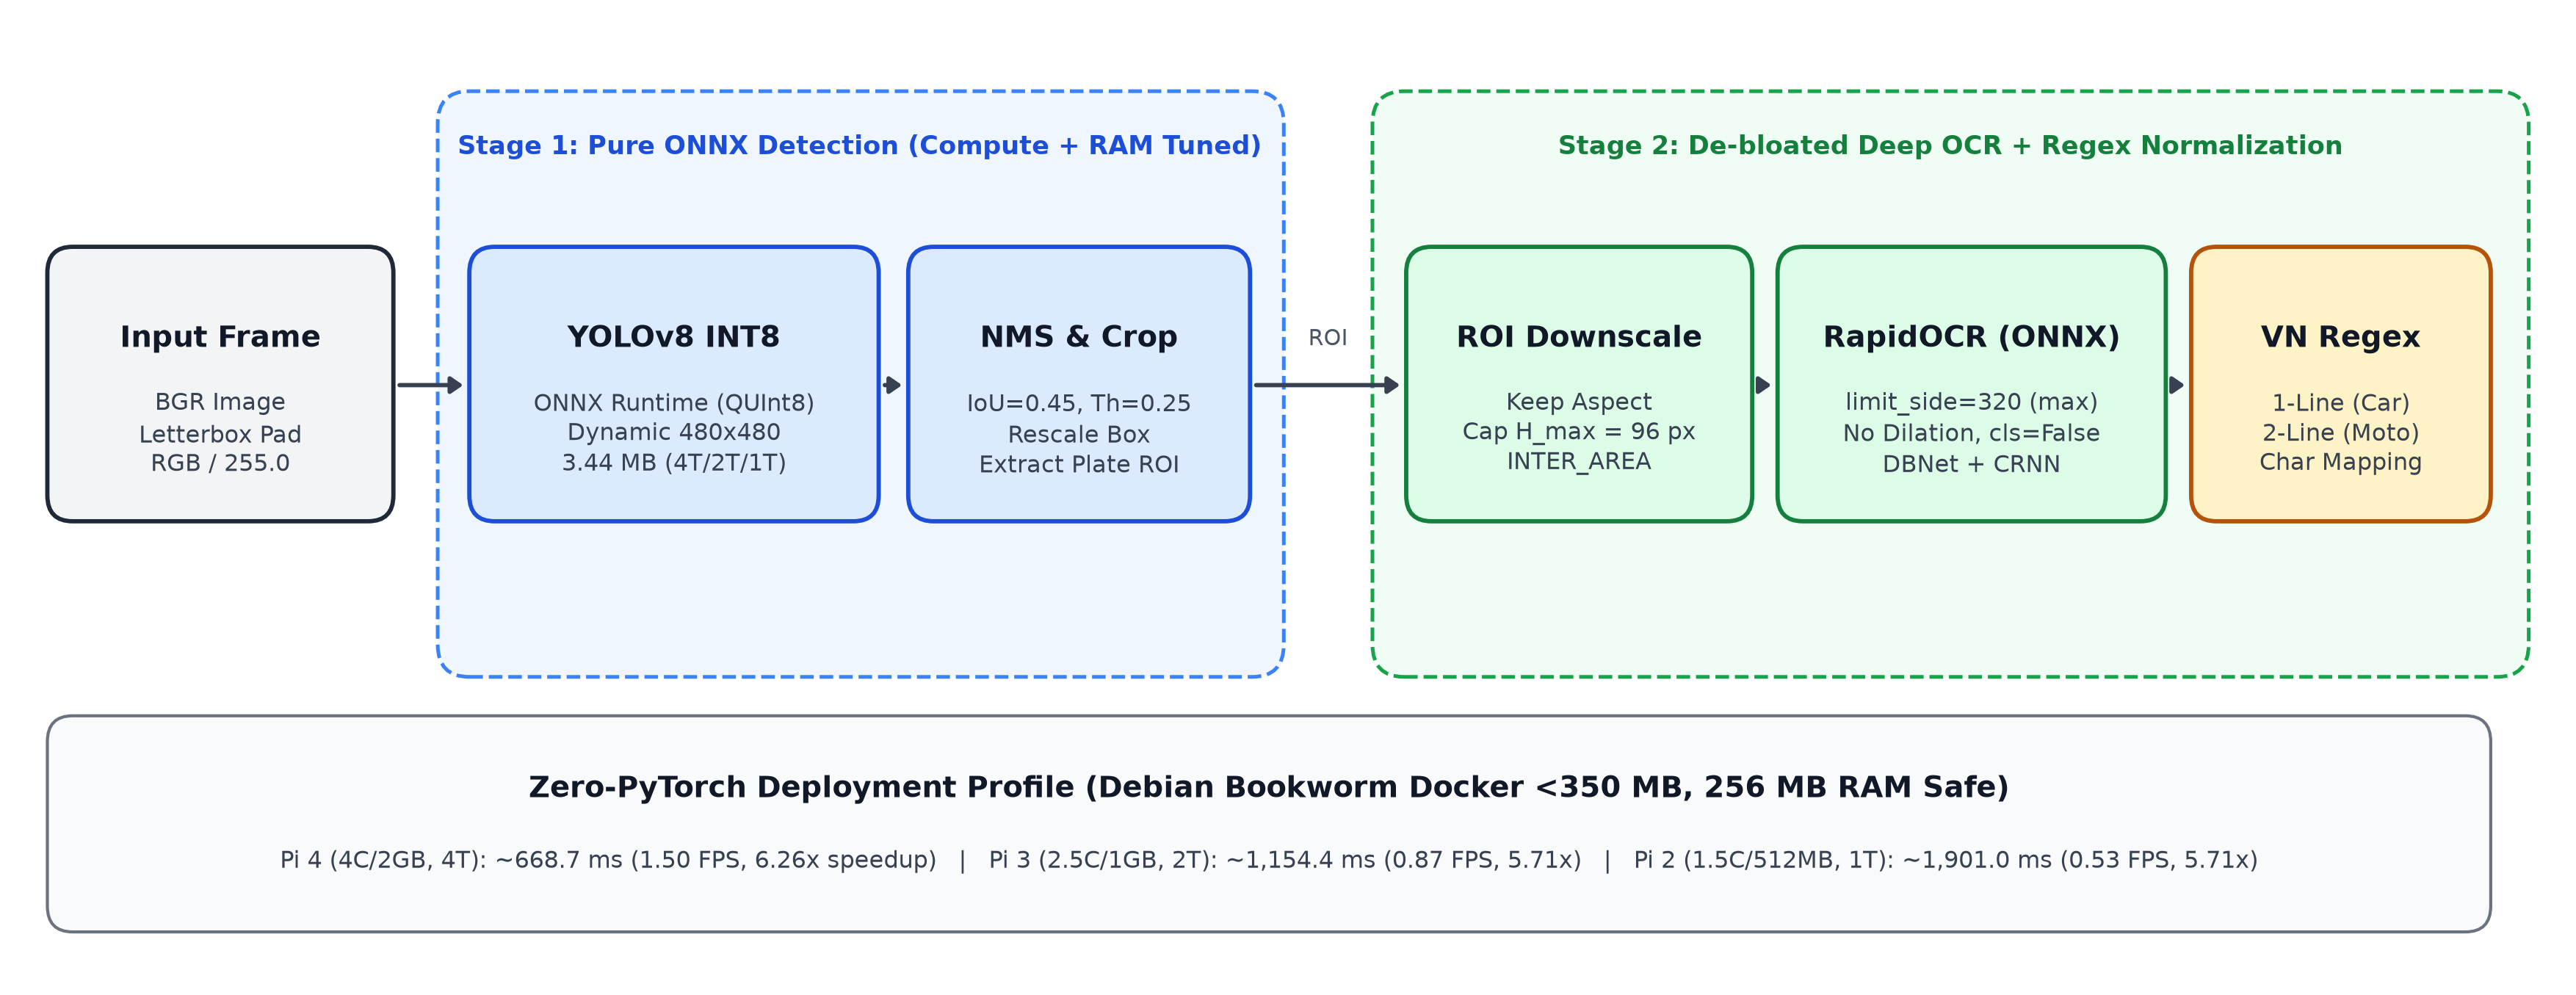
\includegraphics[width=\textwidth]{figures/architecture_pipeline.png}
    \caption{Optimized zero-PyTorch two-stage edge ALPR pipeline, integrating dynamic $480\times 480$ YOLOv8 INT8 detection, hardware-matched intra-op threading, adaptive $H_{\max}=96$\,px ROI downscaling, de-bloated RapidOCR DBNet/CRNN inference, and Vietnamese 1-line/2-line regex normalization.}\label{fig:architecture}
\end{figure}

\subsection{Zero-PyTorch ONNX Conversion, Pruning, and INT8 Quantization}\label{subsec:compression}
Standard Ultralytics PyTorch inference requires installing \texttt{torch} and \texttt{ultralytics} ($>1.5$\,GB disk footprint) and allocates 330.96\,MB resident RAM upon model initialization, causing immediate Linux OOM termination on 256\,MB--512\,MB edge boards. In \texttt{pipeline/optimize.py}, we convert the YOLOv8n detector (\texttt{best.pt}, 5.97\,MB) to simplified ONNX graph format (opset~18 via \texttt{onnxslim}) and apply ONNX Runtime dynamic weight-only \texttt{QUInt8} quantization (\texttt{quantize\_dynamic}). An initial static $640\times 640$ ONNX graph (11.70\,MB) compressed to 3.20\,MB ($-72.6\%$), while the subsequent dynamic-input ONNX export supporting arbitrary $(H, W)$ (11.94\,MB) compressed to 3.44\,MB ($-71.2\%$). We also implement 25\% L1-norm unstructured pruning across all \texttt{Conv2d} layers in PyTorch, attaining 24.91\% weight sparsity (750,112 zeroed parameters in \texttt{best\_pruned.pt}, 11.78\,MB); however, because dense ONNX CPU kernels do not accelerate unstructured sparsity natively without sparse runtimes, production edge deployment uses pure INT8 ONNX weights (\texttt{best\_int8.onnx}) executed strictly with \texttt{onnxruntime}, \texttt{opencv-python-headless}, \texttt{numpy}, \texttt{pillow}, \texttt{psutil}, and \texttt{rapidocr-onnxruntime}.

\subsection{Dynamic Resolution Scaling and Thread Pinning}\label{subsec:scaling}
Since convolutional compute scales quadratically with spatial dimensions $S^2$, we export YOLOv8 with dynamic spatial axes and evaluate scaling $S \in \{640, 512, 480, 384, 320\}$. Letterbox coordinate inversion transforms predicted box $[x_1, y_1, x_2, y_2]$ from network space back to source pixels $(W_0, H_0)$ via scale ratio $r = \min(S/H_0, S/W_0)$ and half-padding offsets $(d_w, d_h)$:
\begin{equation}
    x_{\text{orig}} = \operatorname{clip}\!\left(\operatorname{round}\!\left(\frac{x_{\text{net}} - d_w}{r}\right), 0, W_0\right), \quad
    y_{\text{orig}} = \operatorname{clip}\!\left(\operatorname{round}\!\left(\frac{y_{\text{net}} - d_h}{r}\right), 0, H_0\right).
\end{equation}
Simultaneously, in \texttt{ONNXPlateDetector}, we set \texttt{inter\_op\_num\_threads = 1}, enable full graph optimization (\texttt{ORT\_ENABLE\_ALL}), and pin \texttt{intra\_op\_num\_threads} directly to physical core availability (4 threads for Pi~4, 2 threads for Pi~3, 1 thread for Pi~2/Zero) to eliminate context-switching overhead on weak ARM cores.

\subsection{Eliminating Hidden Deep OCR Over-Processing}\label{subsec:ocr_opt}
Docker resource-limit stress tests (Section~\ref{subsec:exp_bottleneck}) uncovered that even after cutting detector latency below $\sim$280\,ms on Pi~4, total pipeline latency remained 5.34--34.40\,s, with RapidOCR accounting for 85\%--95\% of runtime. Inspecting \texttt{rapidocr\_onnxruntime} internals revealed a severe implicit bottleneck: its default DBNet text detector enforces \texttt{det\_limit\_side\_len = 736} with \texttt{det\_limit\_type = 'min'}. Consequently, every compact cropped license plate ROI (typically $90\times 45$\,px to $180\times 80$\,px) was silently upscaled $5\times$--$10\times$ so its shorter edge reached 736\,px, forcing DBNet to process multi-megapixel feature maps on a Raspberry Pi CPU.

We eliminate this redundant computation in \texttt{pipeline/recognizer\_rapid.py} through four synergistic changes that require zero model retraining:
\begin{enumerate}
    \item \textbf{Disable angle classification (\texttt{use\_cls=False}):} Security-gate cameras maintain upright orientation, skipping $180^\circ$ text-angle classification saves 0.87--2.28\,s per frame across Pi tiers.
    \item \textbf{Invert DBNet resize constraint (\texttt{det\_limit\_side\_len=320}, \texttt{det\_limit\_type='max'}):} Caps the longest edge at 320\,px rather than stretching the short edge to 736\,px, suppressing implicit multi-megapixel upscaling.
    \item \textbf{Remove morphological dilation (\texttt{det\_donot\_use\_dilation=True}):} Avoids extra binary post-filtering passes over DBNet probability maps.
    \item \textbf{Adaptive ROI downscaling ($H_{\max}=96$\,px):} Whenever cropped ROI height $h > 96$\,px, we downsample prior to OCR via area interpolation:
    \begin{equation}
        (w', h') = \left(\max\!\left(16, \left\lfloor w \cdot \frac{96}{h} \right\rfloor\right), \, 96\right).
    \end{equation}
\end{enumerate}

\subsection{Vietnamese Dual-Line Post-Processing}\label{subsec:postprocess}
Vietnamese registration plates follow structured prefixes comprising a two-digit province code ($11$--$99$), registration series characters, and four- or five-digit registration numbers arranged either on a single row (cars) or stacked across two rows (motorcycles and square car plates). In \texttt{pipeline/postprocess.py}, raw recognized text fragments are stripped of non-alphanumeric symbols and uppercased into sequence $c$. Concatenated tokens matching 5-digit pattern \verb|^([0-9]{2}[A-Z0-9]{1,3})([0-9]{3})([0-9]{2})$| or 4-digit pattern \verb|^([0-9]{2}[A-Z0-9]{1,3})([0-9]{4})$| are normalized into canonical \texttt{SS-NNN.NN} and \texttt{SS-NNNN} forms. When RapidOCR returns $\ge 2$ separate line segments $(l_1, l_2)$, $l_1$ is treated as the province/series header and $l_2$ passes through visual character-to-digit mapping (\texttt{O/D/Q$\rightarrow$0}, \texttt{I/L$\rightarrow$1}, \texttt{Z$\rightarrow$2}, \texttt{E$\rightarrow$3}, \texttt{A$\rightarrow$4}, \texttt{S$\rightarrow$5}, \texttt{G$\rightarrow$6}, \texttt{T$\rightarrow$7}, \texttt{B/R$\rightarrow$8}) before formatting the lower numeric group.

\section{Experimental Setup and Reproducible Benchmark Protocol}\label{sec:setup}

\subsection{Hardware Simulation Profiles and Host Environment}\label{subsec:env}
Phase~1--5 hardware optimization experiments were conducted inside lightweight Debian Bookworm Docker containers (\texttt{Dockerfile.rpi4}, image size $<350$\,MB) using strict Linux cgroup CPU and memory quotas to emulate three embedded tiers:
\begin{itemize}
    \item \textbf{Raspberry Pi~4 profile:} 4.0 CPU cores, 2048\,MB RAM (\texttt{threads=4}).
    \item \textbf{Raspberry Pi~3 profile:} 2.5 CPU cores (2.0 cores in stress test), 1024\,MB RAM (\texttt{threads=2}).
    \item \textbf{Raspberry Pi~2 / Zero~2W profile:} 1.5 CPU cores (1.0 core in stress test), 512\,MB RAM, plus an extreme 256\,MB RAM survival test (\texttt{threads=1}).
\end{itemize}
Note that cgroup-throttled \texttt{x86\_64} Docker execution isolates CPU core and RAM budgets accurately, but reflects relative scaling ratios rather than exact ARM Cortex-A72/A53 clock-for-clock instructions.

Full Phase~6 batch evaluation (\texttt{evaluation/run\_benchmark.py}) ran on a Windows~11 AMD64 host (\texttt{Python 3.14.5}, \texttt{onnxruntime 1.30.0}, \texttt{opencv-python-headless 4.13.0.92}, \texttt{rapidocr-onnxruntime 1.2.3}, \texttt{threads=4}) using unified detector confidence $\tau_{\text{det}}=0.001$ (retaining low-confidence proposals for exact all-points AP@50 integration), OCR confidence gating $\tau_{\text{ocr}}=0.25$, and $\tau_{\text{NMS}}=0.45$. Process memory (MiB) was sampled at 10\,ms intervals via \texttt{psutil}. Cross-platform reproducibility was further verified inside \texttt{Dockerfile.benchmark} (Debian Linux headless with \texttt{libgl1}, \texttt{libglib2.0-0}, \texttt{libgomp1}, and explicit removal of GUI \texttt{opencv-python} to prevent \texttt{libxcb.so.1} import failures).

\subsection{Two-Tier Dataset Strategy and Synthetic Perturbation Suite}\label{subsec:datasets}
To prevent both simulated overfitting and opaque dataset reporting, we construct a two-tier evaluation suite (\texttt{0} overlapping filenames between sources; \texttt{0} \texttt{UNKNOWN} labels):
\begin{enumerate}
    \item \textbf{Source~A (Clean Controlled Baseline, $N=300$):} Clean $640\times 640$ images balanced evenly between cars (150 images) and motorcycles (150 images), corresponding to 135 one-line plates and 165 two-line plates. Clean baseline labels combine verified COCO-format bounding boxes~\cite{lin2014coco} with exploratory OCR annotations (\texttt{labels\_verified=false}).
    \item \textbf{Source~A Synthetic Robustness Cohort ($N=100$ subset $\times 30$ variants):} Using \texttt{evaluation/corruptions.py} (\texttt{seed=42}), we generate all 10 realistic perturbation scenarios across 3 monotonic severity levels (Table~\ref{tab:corruptions_spec}), creating 9,000 corrupted images from all 300 Source~A plates. Under \texttt{perspective\_tilt}, bounding boxes are reprojected via the exact $3\times 3$ homography matrix $H$ and linked via explicit \texttt{original\_annotation\_id} lineage (\texttt{0} dropped boxes across all $300\times 3$ transforms). To evaluate the full $64$-cell matrix sequentially within a single-process run, we sample a fixed cohort of $N=100$ Source~A plates (\texttt{seed=42}, preserving source balance with 54 cars / 46 motorcycles and 47 one-line / 53 two-line plates, shared cohort hash \texttt{d62623e9359cba80}), evaluated alongside clean Source~A and Source~B at Pareto resolution $480\times 480$.
    \item \textbf{Source~B (Real-World Adverse Field Sanity Check, $N=60$):} Sixty independent field captures stratified equally into four real-world degradation slices (15 images per slice): \emph{Low Light} (mean gray brightness $61.8$, range $51.8$--$67.7$; 12/15 two-line), \emph{Motion / Defocus Blur} (mean Laplacian sharpness $219.0$; 12/15 two-line), \emph{High Glare / Overexposure} (mean brightness $145.6$; 13/15 two-line), and \emph{Geometry / Perspective Tilt} (15/15 two-line motorcycle plates). Overall, 52 of 60 Source~B plates (86.7\%) are two-line plates.
\end{enumerate}

\begin{table}[t]
\centering
\caption{Summary of the 10 synthetic corruption scenarios evaluated across severity Levels 1, 2, and 3.}\label{tab:corruptions_spec}
\footnotesize
\setlength{\tabcolsep}{3pt}
\begin{tabular}{@{}>{\raggedright\arraybackslash}p{2.5cm}>{\raggedright\arraybackslash}p{2.85cm}>{\raggedright\arraybackslash}p{6.7cm}@{}}
\toprule
\textbf{Category} & \textbf{Scenario ID} & \textbf{Physical Transform Across Levels 1 $\rightarrow$ 3} \\
\midrule
\multirow{3}{*}{Optics \& Light} & \texttt{low\_light} & HSV Value scaling + gamma darkening ($\gamma < 0.6$) \\
 & \texttt{overexposure} & Localized Gaussian glare blob over plate neighborhood \\
 & \texttt{uneven\_shadows} & Directional alpha mask reducing local luminance 40\%--60\% \\
\midrule
\multirow{2}{*}{Blur \& Focus} & \texttt{motion\_blur} & Directional linear motion kernel ($k \in \{7, 15, 25\}$) \\
 & \texttt{defocus\_blur} & Isotropic Gaussian blur ($k \in \{5, 9, 15\}$) \\
\midrule
\multirow{3}{*}{Weather \& Channel} & \texttt{rain\_streaks} & Translucent directional rain streaks ($60^\circ$--$80^\circ$) \\
 & \texttt{sensor\_noise} & Zero-mean additive Gaussian noise ($\sigma \in \{15, 30, 50\}$) \\
 & \texttt{jpeg\_compression} & Low-bitrate JPEG re-encoding ($Q \in \{30, 15, 5\}$) \\
\midrule
\multirow{2}{*}{Geometry \& Occl.} & \texttt{perspective\_tilt} & Homography warp ($\approx 15^\circ, 30^\circ, 45^\circ$) + box reprojection \\
 & \texttt{partial\_occlusion} & Random dark blotches/scratches masking 5\%--15\% plate area \\
\bottomrule
\end{tabular}
\end{table}

\subsection{Formal Quantitative Metrics}\label{subsec:metrics}
All evaluation quantities are implemented in \texttt{evaluation/metrics.py} using unified matching rules:
\begin{itemize}
    \item \textbf{Detection (mAP@50, Precision, Recall):} Detections within the same image and class are greedily matched to ground-truth boxes by descending confidence with $\text{IoU} \ge 0.50$. Precision and Recall evaluate predictions above $\tau_{\text{ocr}}=0.25$, while AP@50 integrates the all-points monotonically interpolated precision envelope across all candidate confidences $\ge \tau_{\text{det}}=0.001$.
    \item \textbf{End-to-End Exact Match (EM) and Character Error Rate (CER):} After NFC normalization, uppercasing, and removal of whitespace, dots, and hyphens, one-to-one box matching pairs predicted strings $\hat{s}_i$ to ground truth $s_i$. Missed ground-truth plates receive $\hat{s}_i = \varnothing$ (counting all $|s_i|$ characters as deletions). With Levenshtein edit distance $d(\hat{s}_i, s_i)$~\cite{levenshtein1966binary}:
    \begin{equation}
        \text{EM} = \frac{1}{N}\sum_{i=1}^{N} \mathbb{I}[\hat{s}_i = s_i] \times 100\%, \qquad
        \text{CER} = \frac{\sum_{i=1}^{N} d(\hat{s}_i, s_i)}{\sum_{i=1}^{N} |s_i|}.
    \end{equation}
    Both metrics are computed overall and sliced separately over \texttt{one\_line} vs.\ \texttt{two\_line} plates.
    \item \textbf{Robustness Degradation and Localization Drift:} Relative EM degradation and bounding-box drift $\Delta\text{IoU}$ are defined over matched plate identities on clean ($B_{\text{clean}}$) and corrupted ($B_{\text{corr}}$) pairs (after projecting $B_{\text{clean}}$ through $H$ under \texttt{perspective\_tilt}):
    \begin{equation}
        \text{Deg} = \frac{\text{EM}_{\text{clean}} - \text{EM}_{\text{corr}}}{\text{EM}_{\text{clean}}} \times 100\%, \qquad
        \Delta\text{IoU} = 1 - \text{IoU}\!\left(B_{\text{clean}}, B_{\text{corr}}\right).
    \end{equation}
\end{itemize}

\section{Experimental Results and Analysis}\label{sec:results}

\subsection{Model Compression and Memory-to-Compute Shift (Phases 2--3)}\label{subsec:exp_bottleneck}
Table~\ref{tab:compression_ram} summarizes detector compression gains measured via \texttt{verify\_comparison.py} and \texttt{benchmark\_edge\_resources.py}. Moving from PyTorch FP32 (\texttt{best.pt}) to Pure ONNX INT8 cuts initialization RAM by \textbf{83.8\%} (330.96\,MB $\rightarrow$ 53.61\,MB) while keeping bounding-box IoU consistency at \textbf{97.8\%} on reference samples. Note that the initial static ONNX graph (11.70\,MB $\rightarrow$ 3.20\,MB, $-72.6\%$) and the dynamic-shape ONNX graph used in Phases~4--6 (11.94\,MB $\rightarrow$ 3.44\,MB, $-71.2\%$) achieve essentially identical weight compression.

\begin{table}[t]
\centering
\caption{Model compression, weight footprint, initialization RAM, and bounding-box fidelity (Phase~2).}\label{tab:compression_ram}
{\fontsize{6.4pt}{7.8pt}\selectfont\setlength{\tabcolsep}{1.8pt}
\begin{tabular}{@{}>{\raggedright\arraybackslash}p{2.95cm}cccc@{}}
\toprule
\textbf{Detector Variant} & \textbf{Weight Size} & \textbf{Compression} & \textbf{Init RAM} & \textbf{Fidelity vs.\ FP32} \\
\midrule
PyTorch Baseline (\texttt{best.pt}) & 5.97\,MB & Baseline & 330.96\,MB & IoU 100\%, Conf 91.7\% \\
Pruned L1 25\% (\texttt{best\_pruned.pt}) & 11.78\,MB & 24.91\% sparsity & -- & Conf 90.5\% (750k zeros) \\
ONNX FP32\newline(static / dynamic) & 11.70/11.94\,MB & Graph fused & $\sim$110.0\,MB & IoU 99.1\%, Conf 94.3\% \\
\textbf{ONNX INT8}\newline\textbf{(static / dynamic)} & \textbf{3.20/3.44\,MB} & \textbf{$-72.6\%$/$-71.2\%$} & \textbf{53.61\,MB ($-83.8\%$)} & \textbf{IoU 97.8\%, Conf 92.2\%} \\
\bottomrule
\end{tabular}%
}
\end{table}

Table~\ref{tab:stress_test} reports Docker cgroup stress-testing results prior to OCR de-bloating. Pure ONNX INT8 executes safely without OOM termination all the way down to \textbf{256\,MB RAM} (a single-core legacy ceiling where PyTorch crashes during load). Crucially, however, while detector execution takes only 281.34\,ms (Pi~4) to 1,000.90\,ms (extreme single-core), default RapidOCR dominates runtime at 5.06\,s to 33.41\,s (\textbf{85\%--95\%} of pipeline latency), confirming a sharp transition from memory-bound to compute-bound behavior.

\begin{table}[t]
\centering
\caption{Docker cgroup memory/CPU stress-test profiling before OCR optimization (Phase~3).}\label{tab:stress_test}
\footnotesize
\setlength{\tabcolsep}{4pt}
\begin{tabular}{@{}lccccc@{}}
\toprule
\textbf{Emulated Tier} & \textbf{Cgroup Quota} & \textbf{Det (INT8)} & \textbf{Default OCR} & \textbf{Total} & \textbf{OOM} \\
\midrule
Tier 1: RPi 4 & 4.0C / 2048\,MB & 281.34\,ms & 5,060.00\,ms & 5.34\,s & Survived \\
Tier 2: RPi 3 B+ & 2.0C / 1024\,MB & 453.68\,ms & 9,486.00\,ms & 9.94\,s & Survived \\
Tier 3: RPi Zero 2W & 1.0C / 512\,MB & 1,095.84\,ms & 16,574.00\,ms & 17.67\,s & Survived \\
Tier 4: Legacy 256M & 1.0C / 256\,MB & 1,000.90\,ms & 33,406.85\,ms & 34.40\,s & \textbf{0 OOM} \\
\bottomrule
\end{tabular}
\end{table}

\subsection{Resolution Scaling, SIMD Threading, and OCR Speedup (Phases 4--5)}\label{subsec:exp_speedup}
Table~\ref{tab:scaling_threads} isolates detector latency across input resolutions and thread counts. Reducing input resolution from $640\times 640$ to $480\times 480$ accelerates YOLOv8 INT8 by $1.64\times$ (Pi~4), $2.07\times$ (Pi~3), and $1.85\times$ (Pi~2) while actually improving sample confidence from 59.2\% to 60.3\% and keeping 100\% OCR fidelity; conversely, dropping further to $320\times 320$ degrades edge sharpness and confidence (41.7\%). Thread-scaling results further prove that ONNX Runtime \texttt{intra\_op\_num\_threads} must match physical core count: forcing 4 threads onto a 2.5-core (Pi~3) or 1.5-core (Pi~2) quota increases detector latency from 114.28\,ms to 174.01\,ms and from 151.58\,ms to 299.32\,ms, respectively, due to thread synchronization contention.

\begin{table}[t]
\centering
\caption{Dynamic resolution scaling and intra-op thread pinning across edge hardware tiers (Phase~4).}\label{tab:scaling_threads}
{\fontsize{6.8pt}{8.2pt}\selectfont\setlength{\tabcolsep}{1.8pt}
\begin{tabular}{@{}lccccccc@{}}
\toprule
\multirow{2}{*}{\textbf{Emulated Tier}} & \multicolumn{4}{c}{\textbf{Resolution Scaling (ms / Speedup vs.\ 640)}} & \multicolumn{3}{c}{\textbf{Threads @ 480 (ms)}} \\
\cmidrule(lr){2-5} \cmidrule(l){6-8}
 & \texttt{640} & \texttt{480} (Pareto) & \texttt{384} & \texttt{320} & \texttt{1T} & \texttt{2T} & \texttt{4T} \\
\midrule
RPi 4 (4C/2G) & 187.43 & \textbf{114.17 ($1.64\times$)} & 68.64 ($2.73\times$) & 59.94 ($3.13\times$) & 154.54 & 118.12 & \textbf{100.32} \\
RPi 3 (2.5C/1G) & 236.63 & \textbf{114.33 ($2.07\times$)} & 77.39 ($3.06\times$) & 60.06 ($3.94\times$) & 155.56 & \textbf{114.28} & 174.01 \\
RPi 2 (1.5C/512M) & 296.99 & \textbf{160.54 ($1.85\times$)} & 102.22 ($2.91\times$) & 70.57 ($4.21\times$) & \textbf{151.58} & 161.50 & 299.32 \\
\bottomrule
\end{tabular}%
}
\end{table}

Applying our four-step OCR de-bloating strategy (Section~\ref{subsec:ocr_opt}) slashes OCR latency by \textbf{$5.85\times$} on Pi~4 (3,322.86\,ms $\rightarrow$ 568.42\,ms), \textbf{$4.89\times$} on Pi~3 (5,081.26\,ms $\rightarrow$ 1,040.14\,ms), and \textbf{$4.71\times$} on Pi~2 (8,240.25\,ms $\rightarrow$ 1,749.40\,ms) with 100\% OCR parity on benchmark plates (\texttt{68G1-668.86}, \texttt{51A-222.22}). Combining INT8 $480\times 480$ detection with tuned RapidOCR drops total end-to-end latency from 4,184.24\,ms to \textbf{668.74\,ms ($\sim 1.50$\,FPS, $6.26\times$ overall speedup)} on Pi~4, from 6,597.99\,ms to \textbf{1,154.42\,ms ($5.71\times$)} on Pi~3, and from 10,856.81\,ms to \textbf{1,900.98\,ms ($5.71\times$)} on Pi~2, as depicted in Fig.~\ref{fig:rpi_speedup}.

\begin{figure}[t]
    \centering
    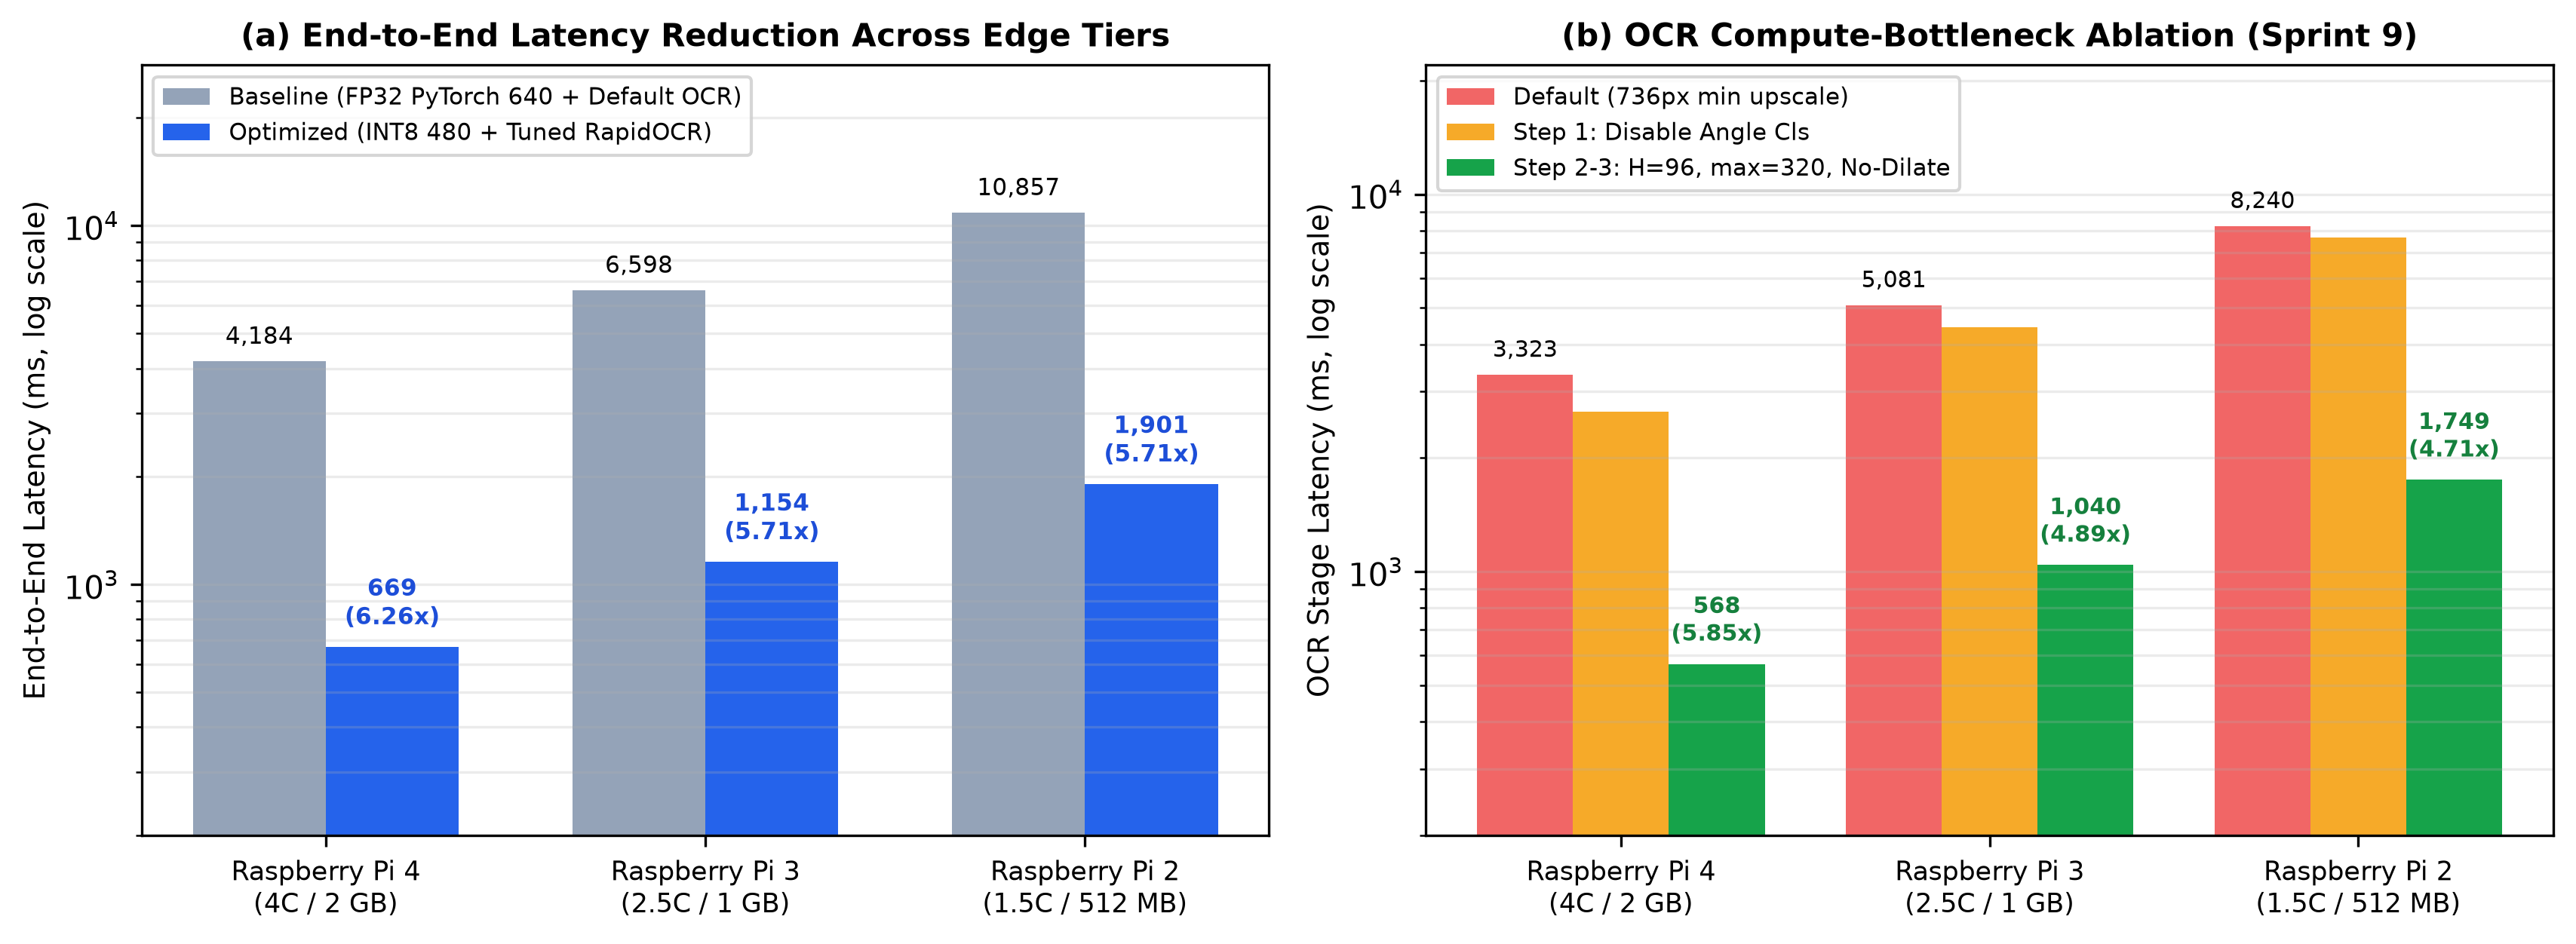
\includegraphics[width=\textwidth]{figures/rpi_end_to_end_speedup.png}
    \caption{Phase~5 throughput breakthroughs under Raspberry Pi cgroup profiles: (a) overall end-to-end latency reduction ($5.71\times$--$6.26\times$ speedup) and (b) stage-wise OCR ablation proving that eliminating DBNet 736\,px minimum-side upscaling yields a $4.71\times$--$5.85\times$ speedup.}\label{fig:rpi_speedup}
\end{figure}

\subsection{Full Clean Multi-Resolution Baseline (Source A \& Source B)}\label{subsec:exp_clean}
Table~\ref{tab:clean_full} presents the complete 12-run clean multi-resolution benchmark across all 300 Source~A and 60 Source~B plates (2,160 total inferences on the \texttt{x86\_64} host, \texttt{threads=4}), accompanied by Fig.~\ref{fig:clean_tradeoff}. Three structural findings emerge:
\begin{enumerate}
    \item \textbf{Resolution $480\times 480$ improves precision while preserving EM:} On Source~A ($N=300$), scaling from $640$ to $480$ reduces detector false positives by over two-thirds, boosting Precision from 85.37\%--85.80\% to \textbf{94.44\%--94.74\%}, while holding mAP@50 near 96\% (96.32\% FP32, 95.94\% INT8) and overall EM above 70\% (72.33\% FP32, 70.33\% INT8). Further scaling to $320$ cuts Recall on small motorcycle plates (lowering moto mAP@50 from 91.9\%--92.5\% at 640 down to 88.4\%--90.1\% at 320).
    \item \textbf{Car (1-line) vs.\ Motorcycle (2-line) disparity:} Across all resolutions on Source~A, cars ($n=150$) attain \textbf{100.00\% mAP@50} (640 and 480) and \textbf{94.00\%--95.33\% EM} (\texttt{one\_line} EM 95.56\%--97.04\%, CER 0.0037--0.0112). Motorcycles ($n=150$, \texttt{two\_line}), by contrast, achieve 88.37\%--92.52\% mAP@50 yet drop to \textbf{42.00\%--50.67\% EM} (CER 0.205--0.315), establishing two-line stacked recognition as the primary accuracy bottleneck.
    \item \textbf{x86 AVX2 vs.\ ARM quantization trade-off:} On the desktop \texttt{x86\_64} host, \texttt{QUInt8} detection executes slower than FP32 (e.g., 140.27\,ms vs.\ 95.07\,ms at 480 on Source~A) because standard AVX2 favors FP32 vector instructions when VNNI INT8 kernels are absent, forcing per-op dequantization overhead. Nevertheless, INT8 substantially lowers peak memory (117.21\,MiB vs.\ 335.07\,MiB at 480; noting that sequential in-process RSS reuse attenuates later cell baselines) and yields higher mAP@50 on the hard real-world Source~B dataset across every resolution (65.95\% vs.\ 63.10\% at 640).
\end{enumerate}

\begin{table}[t]
\centering
\caption{Full clean multi-resolution benchmark across Source~A (SA, $n=300$) and Source~B (SB, $n=60$) on \texttt{x86\_64} CPU (4T). 1L/2L denote one-line/two-line EM; latency reports detection, OCR, and end-to-end total means.}\label{tab:clean_full}
{\fontsize{6.6pt}{8.0pt}\selectfont\setlength{\tabcolsep}{1.5pt}
\begin{tabular}{@{}llc@{\hspace{5pt}}rrrrrrrrrr@{}}
\toprule
\textbf{Src} & \textbf{Mdl} & \textbf{Res} & \multicolumn{1}{c}{\textbf{mAP}} & \textbf{Prec.} & \textbf{Rec.} & \textbf{EM} & \textbf{1L} & \textbf{2L} & \textbf{CER} & \textbf{Det} & \textbf{OCR} & \textbf{Total} \\
($N$) & & & \multicolumn{1}{c}{(@50\%)} & (\%) & (\%) & (\%) & (\%) & (\%) & & (ms) & (ms) & (ms/FPS) \\
\midrule
SA (300) & FP32 & 640 & 96.91 & 85.37 & 95.33 & 71.00 & 97.04 & 49.70 & 0.1128 & 112.76 & 82.56 & 207.58/4.82 \\
SA (300) & FP32 & 480 & 96.32 & 94.44 & 90.67 & 72.33 & 95.56 & 53.33 & 0.1414 & 95.07 & 69.15 & 172.04/5.81 \\
SA (300) & FP32 & 320 & 95.10 & 93.99 & 88.67 & 68.33 & 96.30 & 45.45 & 0.1679 & 58.59 & 60.16 & 122.74/8.15 \\
SA (300) & INT8 & 640 & 96.57 & 85.80 & 94.67 & 70.67 & 96.30 & 49.70 & 0.1172 & 244.84 & 91.32 & 347.40/2.88 \\
SA (300) & INT8 & 480 & 95.94 & 94.74 & 90.00 & 70.33 & 96.30 & 49.09 & 0.1510 & 140.27 & 70.00 & 217.34/4.60 \\
SA (300) & INT8 & 320 & 95.54 & 97.05 & 87.67 & 68.67 & 96.30 & 46.06 & 0.1696 & 104.52 & 65.61 & 174.45/5.73 \\
\midrule
SB (60) & FP32 & 640 & 63.10 & 73.47 & 60.00 & 36.67 & 62.50 & 32.69 & 0.5169 & 148.13 & 70.96 & 232.66/4.30 \\
SB (60) & FP32 & 480 & 60.70 & 75.00 & 50.00 & 30.00 & 37.50 & 28.85 & 0.5753 & 96.17 & 51.06 & 157.10/6.37 \\
SB (60) & FP32 & 320 & 54.68 & 84.85 & 46.67 & 35.00 & 50.00 & 32.69 & 0.5663 & 52.24 & 50.59 & 107.34/9.32 \\
SB (60) & INT8 & 640 & \textbf{65.95} & 78.72 & \textbf{61.67} & \textbf{38.33} & 62.50 & \textbf{34.62} & \textbf{0.4652} & 227.86 & 61.31 & 303.98/3.29 \\
SB (60) & INT8 & 480 & 62.11 & 76.92 & 50.00 & 28.33 & 37.50 & 26.92 & 0.5910 & 129.88 & 53.94 & 191.82/5.21 \\
SB (60) & INT8 & 320 & 56.40 & 87.10 & 45.00 & 31.67 & 25.00 & 32.69 & 0.5843 & 83.83 & 45.44 & 132.37/7.55 \\
\bottomrule
\end{tabular}%
}
\end{table}

\begin{figure}[t]
    \centering
    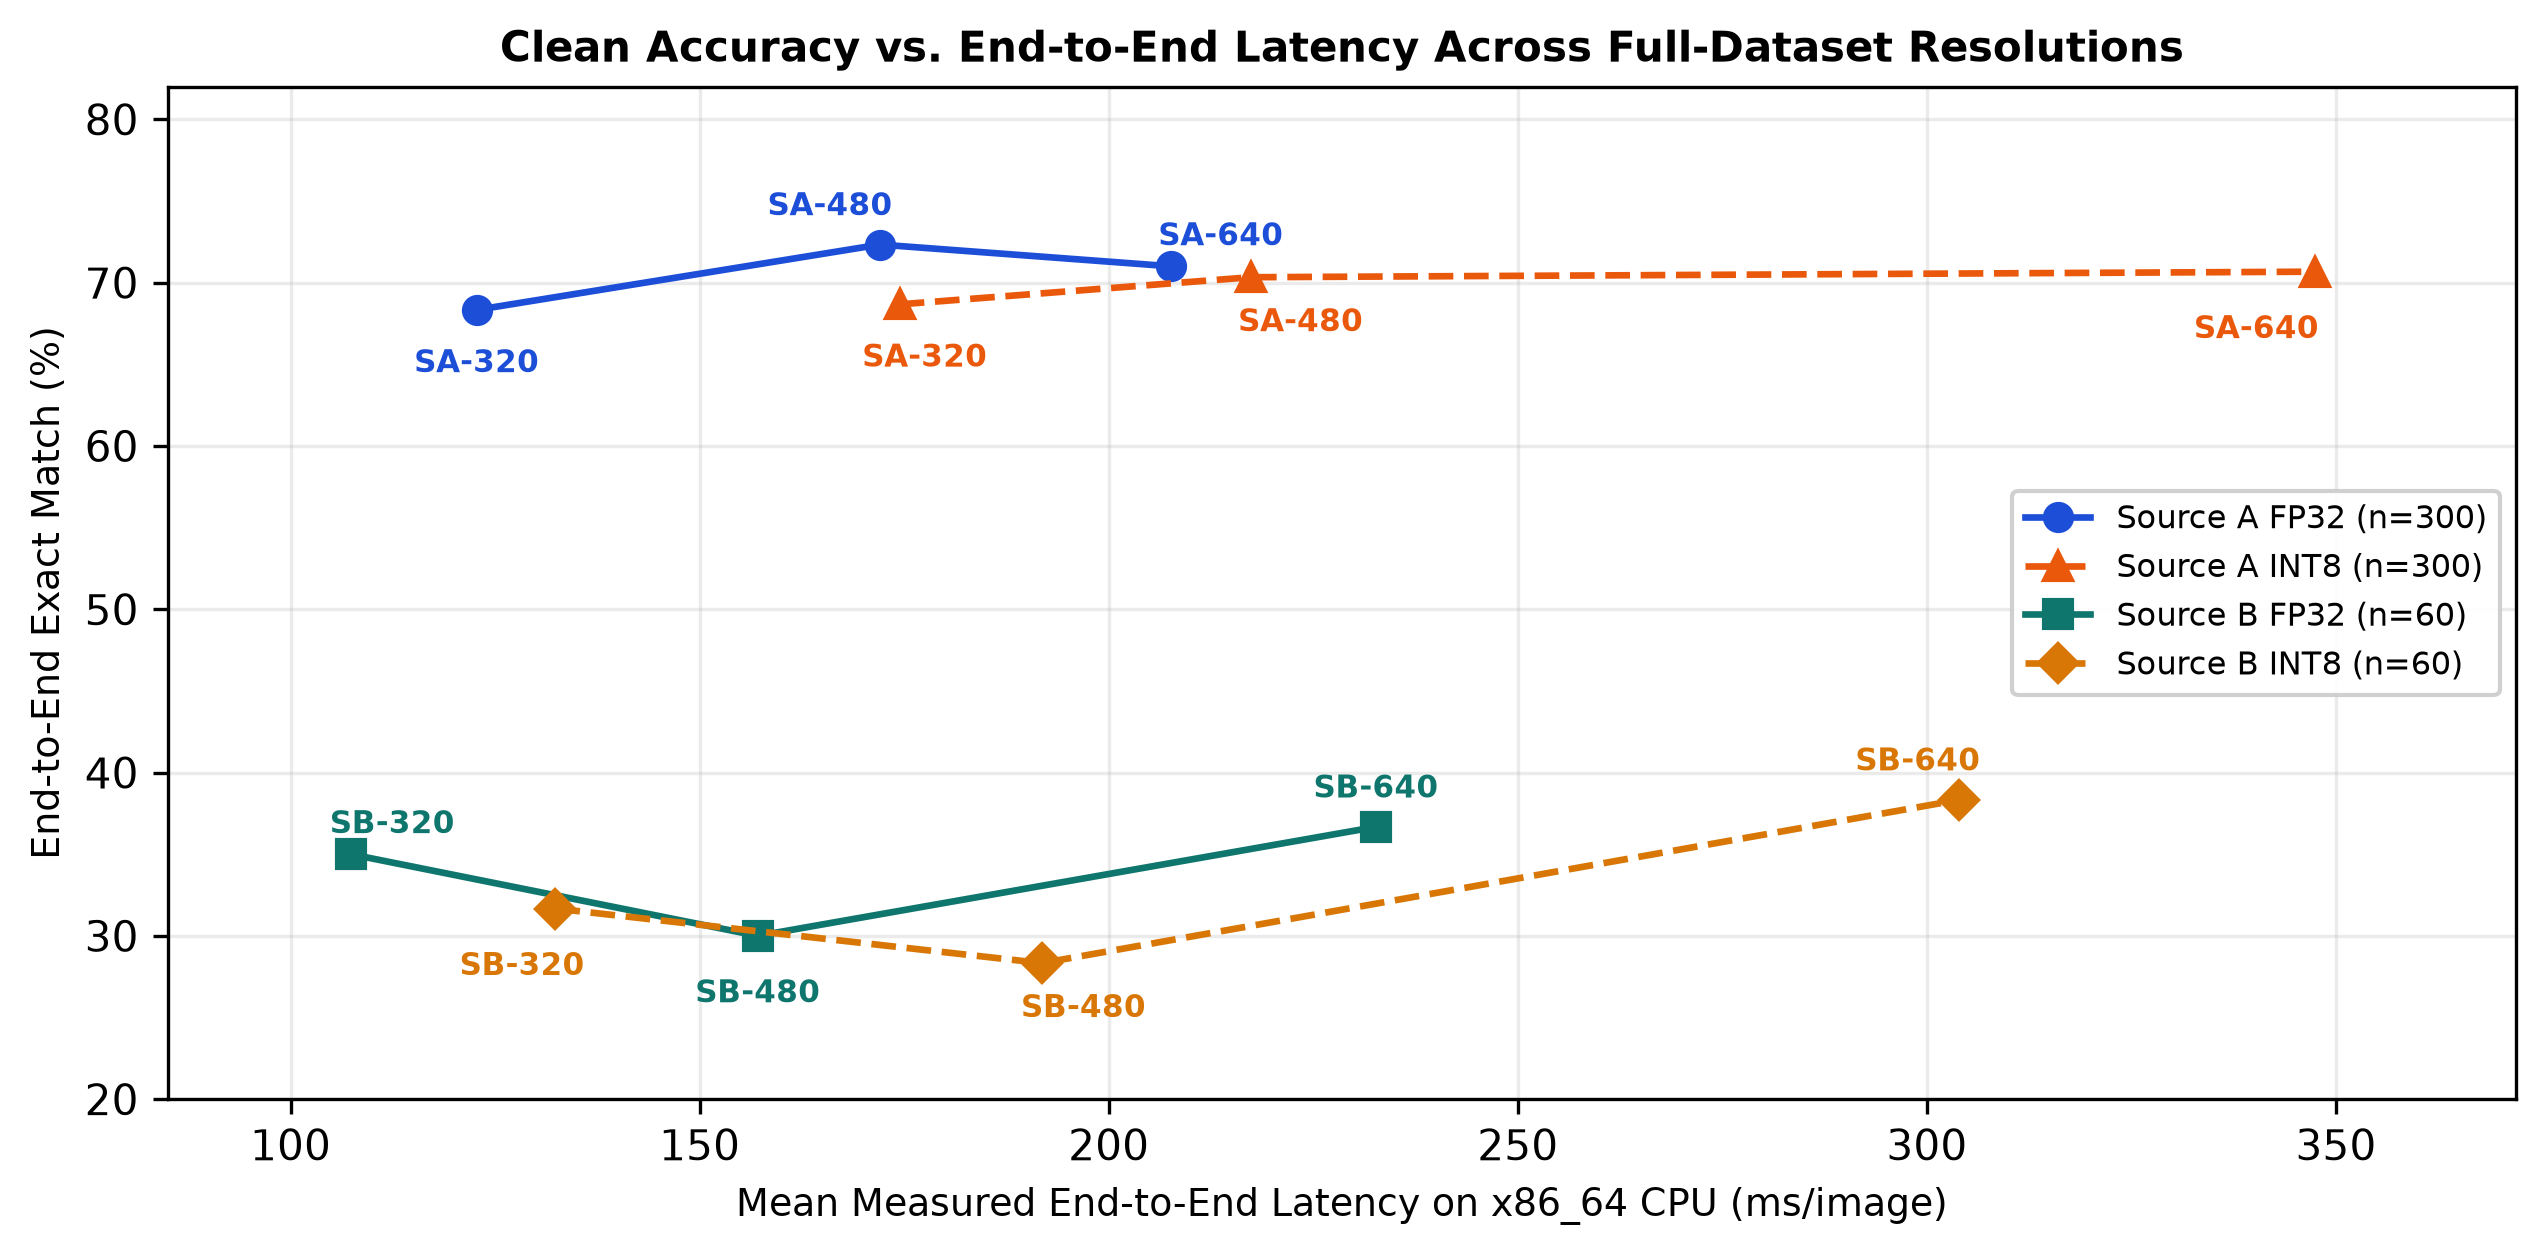
\includegraphics[width=0.92\textwidth]{figures/clean_accuracy_latency.png}
    \caption{Clean accuracy vs.\ measured mean end-to-end latency on \texttt{x86\_64} CPU across all 12 full-dataset configurations ($N=300$ Source~A and $N=60$ Source~B at $640$, $480$, and $320$).}\label{fig:clean_tradeoff}
\end{figure}

\subsection{Ten-Corruption Robustness Matrix: FP32 vs.\ INT8 Parity}\label{subsec:exp_robustness}
Tables~\ref{tab:robustness_full} and~\ref{tab:robustness_summary} report the full 30-corruption matrix at Pareto resolution $480\times 480$ over the identical $N=100$ Source~A cohort (where clean baseline yields $\text{EM}=74.00\%$ for both models, $\text{mAP@50}=97.84\%$ FP32 vs.\ $97.48\%$ INT8). Figure~\ref{fig:degradation} plots relative degradation trajectories across severity levels 1--3, and Fig.~\ref{fig:radar} displays pairwise FP32 vs.\ INT8 radar envelopes at each severity level.

\begin{table}[t]
\centering
\caption{End-to-end robustness across 10 corruption scenarios and 3 severity levels ($480\times 480$, $N=100$ shared Source~A cohort; clean EM $= 74.00\%$ for both FP32 (F) and INT8 (I)). Percentage signs omitted in columns marked (\%).}\label{tab:robustness_full}
{\fontsize{5.6pt}{6.8pt}\selectfont\setlength{\tabcolsep}{1.1pt}
\begin{tabular}{@{}lc@{\hspace{3.5pt}}rr@{\hspace{3.5pt}}rr@{\hspace{3.5pt}}rr@{\hspace{3.5pt}}rr@{\hspace{3.5pt}}r@{}}
\toprule
 & & \multicolumn{2}{c}{\textbf{mAP@50 (\%)}} & \multicolumn{2}{c}{\textbf{EM (1L/2L) (\%)}} & \multicolumn{2}{c}{\textbf{CER}} & \multicolumn{2}{c}{\textbf{Deg (\%)}} & \textbf{$\Delta$IoU} \\
\cmidrule(lr){3-4} \cmidrule(lr){5-6} \cmidrule(lr){7-8} \cmidrule(lr){9-10}
\textbf{Scenario} & \textbf{L} & \textbf{FP32} & \textbf{INT8} & \textbf{FP32} & \textbf{INT8} & \textbf{FP32} & \textbf{INT8} & \textbf{FP32} & \textbf{INT8} & \textbf{(F/I)} \\
\midrule
\multirow{3}{*}{\texttt{low\_light}} & 1 & 97.97 & 97.66 & 69.0(93.6/47.2) & 70.0(91.5/50.9) & 0.1322 & 0.1432 & 6.76 & 5.41 & .020/.021 \\
 & 2 & 95.53 & 95.03 & 65.0(87.2/45.3) & 67.0(87.2/49.1) & 0.1726 & 0.1628 & 12.16 & 9.46 & .050/.050 \\
 & 3 & 56.58 & 59.75 & 0.0(0.0/0.0) & 0.0(0.0/0.0) & 1.0000 & 1.0000 & 100.00 & 100.00 & .126/.124 \\
\midrule
\multirow{3}{*}{\texttt{overexposure}} & 1 & 97.82 & 97.82 & 74.0(97.9/52.8) & 73.0(95.7/52.8) & 0.1346 & 0.1346 & 0.00 & 1.35 & .006/.010 \\
 & 2 & 97.97 & 97.79 & 63.0(87.2/41.5) & 61.0(85.1/39.6) & 0.1701 & 0.1934 & 14.86 & 17.57 & .032/.031 \\
 & 3 & 51.43 & 50.94 & 5.0(8.5/1.9) & 4.0(6.4/1.9) & 0.8825 & 0.8800 & 93.24 & 94.59 & .213/.226 \\
\midrule
\multirow{3}{*}{\texttt{uneven\_shadows}} & 1 & 97.88 & 97.76 & 71.0(93.6/50.9) & 71.0(93.6/50.9) & 0.1359 & 0.1603 & 4.05 & 4.05 & .016/.019 \\
 & 2 & 95.12 & 95.03 & 69.0(97.9/43.4) & 71.0(95.7/49.1) & 0.1652 & 0.1554 & 6.76 & 4.05 & .034/.034 \\
 & 3 & 91.88 & 91.36 & 63.0(93.6/35.9) & 63.0(93.6/35.9) & 0.2766 & 0.2876 & 14.86 & 14.86 & .046/.048 \\
\midrule
\multirow{3}{*}{\texttt{motion\_blur}} & 1 & 95.85 & 96.00 & 22.0(34.0/11.3) & 23.0(34.0/13.2) & 0.3525 & 0.3525 & 70.27 & 68.92 & .077/.079 \\
 & 2 & 95.74 & 94.12 & 2.0(0.0/3.8) & 2.0(0.0/3.8) & 0.9523 & 0.9547 & 97.30 & 97.30 & .127/.127 \\
 & 3 & 92.46 & 93.09 & 1.0(0.0/1.9) & 1.0(0.0/1.9) & 0.9792 & 0.9743 & 98.65 & 98.65 & .174/.178 \\
\midrule
\multirow{3}{*}{\texttt{defocus\_blur}} & 1 & 97.15 & 97.23 & 62.0(91.5/35.9) & 67.0(93.6/43.4) & 0.1432 & 0.1530 & 16.22 & 9.46 & .039/.040 \\
 & 2 & 93.06 & 93.64 & 34.0(44.7/24.5) & 34.0(48.9/20.8) & 0.3660 & 0.3660 & 54.05 & 54.05 & .101/.103 \\
 & 3 & 82.37 & 82.46 & 2.0(0.0/3.8) & 2.0(0.0/3.8) & 0.9339 & 0.9498 & 97.30 & 97.30 & .157/.158 \\
\midrule
\multirow{3}{*}{\texttt{rain\_streaks}} & 1 & 98.45 & 98.36 & 76.0(95.7/58.5) & 73.0(95.7/52.8) & 0.1200 & 0.1212 & -2.70 & 1.35 & .008/.013 \\
 & 2 & 98.21 & 98.39 & 69.0(93.6/47.2) & 68.0(93.6/45.3) & 0.1506 & 0.1518 & 6.76 & 8.11 & .025/.027 \\
 & 3 & 66.75 & 66.29 & 14.0(25.5/3.8) & 10.0(21.3/0.0) & 0.7650 & 0.7882 & 81.08 & 86.49 & .084/.087 \\
\midrule
\multirow{3}{*}{\texttt{sensor\_noise}} & 1 & 99.61 & 99.31 & 72.0(93.6/52.8) & 66.0(91.5/43.4) & 0.1236 & 0.1395 & 2.70 & 10.81 & .031/.031 \\
 & 2 & 98.35 & 97.67 & 53.0(78.7/30.2) & 52.0(78.7/28.3) & 0.2203 & 0.2485 & 28.38 & 29.73 & .046/.049 \\
 & 3 & 97.44 & 97.23 & 33.0(53.2/15.1) & 37.0(57.5/18.9) & 0.3672 & 0.3758 & 55.41 & 50.00 & .060/.059 \\
\midrule
\multirow{3}{*}{\texttt{jpeg\_compression}} & 1 & 98.08 & 98.10 & 73.0(93.6/54.7) & 72.0(91.5/54.7) & 0.1297 & 0.1200 & 1.35 & 2.70 & .011/.013 \\
 & 2 & 99.03 & 98.78 & 66.0(85.1/49.1) & 68.0(85.1/52.8) & 0.1273 & 0.1310 & 10.81 & 8.11 & .014/.018 \\
 & 3 & 98.22 & 98.56 & 48.0(61.7/35.9) & 48.0(61.7/35.9) & 0.2179 & 0.2326 & 35.14 & 35.14 & .032/.034 \\
\midrule
\multirow{3}{*}{\texttt{perspective\_tilt}} & 1 & 96.36 & 95.65 & 68.0(95.7/43.4) & 69.0(95.7/45.3) & 0.1689 & 0.1775 & 8.11 & 6.76 & .048/.049 \\
 & 2 & 95.35 & 94.95 & 68.0(95.7/43.4) & 63.0(91.5/37.7) & 0.1958 & 0.1983 & 8.11 & 14.86 & .069/.069 \\
 & 3 & 81.37 & 80.44 & 56.0(87.2/28.3) & 57.0(89.4/28.3) & 0.3280 & 0.3207 & 24.32 & 22.97 & .119/.120 \\
\midrule
\multirow{3}{*}{\texttt{partial\_occlusion}} & 1 & 96.95 & 96.99 & 34.0(46.8/22.6) & 28.0(42.6/15.1) & 0.2840 & 0.2950 & 54.05 & 62.16 & .016/.020 \\
 & 2 & 95.04 & 95.29 & 11.0(17.0/5.7) & 12.0(19.2/5.7) & 0.3709 & 0.3709 & 85.14 & 83.78 & .027/.030 \\
 & 3 & 94.05 & 93.63 & 4.0(4.3/3.8) & 1.0(0.0/1.9) & 0.5410 & 0.5667 & 94.59 & 98.65 & .037/.040 \\
\bottomrule
\end{tabular}%
}
\end{table}

\begin{table}[t]
\centering
\caption{Aggregated FP32 vs.\ INT8 robustness parity across severity levels (10 perturbations per level, 3,000 corrupted evaluations per model).}\label{tab:robustness_summary}
\footnotesize
\setlength{\tabcolsep}{1.7pt}
\begin{tabular}{@{}llcccccc@{}}
\toprule
\textbf{Scope} & \textbf{Mdl} & \textbf{Mean mAP} & \textbf{Mean EM} & \textbf{EM 1L / 2L} & \textbf{Mean CER} & \textbf{Mean Deg} & \textbf{$\Delta$(INT8$-$FP32)} \\
 & & (\%) & (\%) & (\%) & & (\%) & (mAP / EM) \\
\midrule
\multirow{2}{*}{Level 1} & FP32 & 97.61 & 62.10 & 83.62 / 43.02 & 0.1725 & 16.08 & \multirow{2}{*}{$-0.12$\,pp / $-0.90$\,pp} \\
 & INT8 & 97.49 & 61.20 & 82.55 / 42.26 & 0.1797 & 17.30 & \\
\midrule
\multirow{2}{*}{Level 2} & FP32 & 96.34 & 50.00 & 68.72 / 33.40 & 0.2891 & 32.43 & \multirow{2}{*}{$-0.27$\,pp / $-0.20$\,pp} \\
 & INT8 & 96.07 & 49.80 & 68.51 / 33.21 & 0.2933 & 32.70 & \\
\midrule
\multirow{2}{*}{Level 3} & FP32 & 81.26 & 22.60 & 33.40 / 13.02 & 0.6291 & 69.46 & \multirow{2}{*}{$+0.12$\,pp / $-0.30$\,pp} \\
 & INT8 & 81.38 & 22.30 & 32.98 / 12.83 & 0.6376 & 69.86 & \\
\midrule
\multirow{2}{*}{\textbf{All 30}} & \textbf{FP32} & \textbf{91.74} & \textbf{44.90} & \textbf{61.91 / 29.81} & \textbf{0.3636} & \textbf{39.32} & \multirow{2}{*}{\textbf{$-0.09$\,pp / $-0.47$\,pp}} \\
 & \textbf{INT8} & \textbf{91.64} & \textbf{44.43} & \textbf{61.35 / 29.43} & \textbf{0.3702} & \textbf{39.95} & \\
\bottomrule
\end{tabular}
\end{table}

\begin{figure}[t]
    \centering
    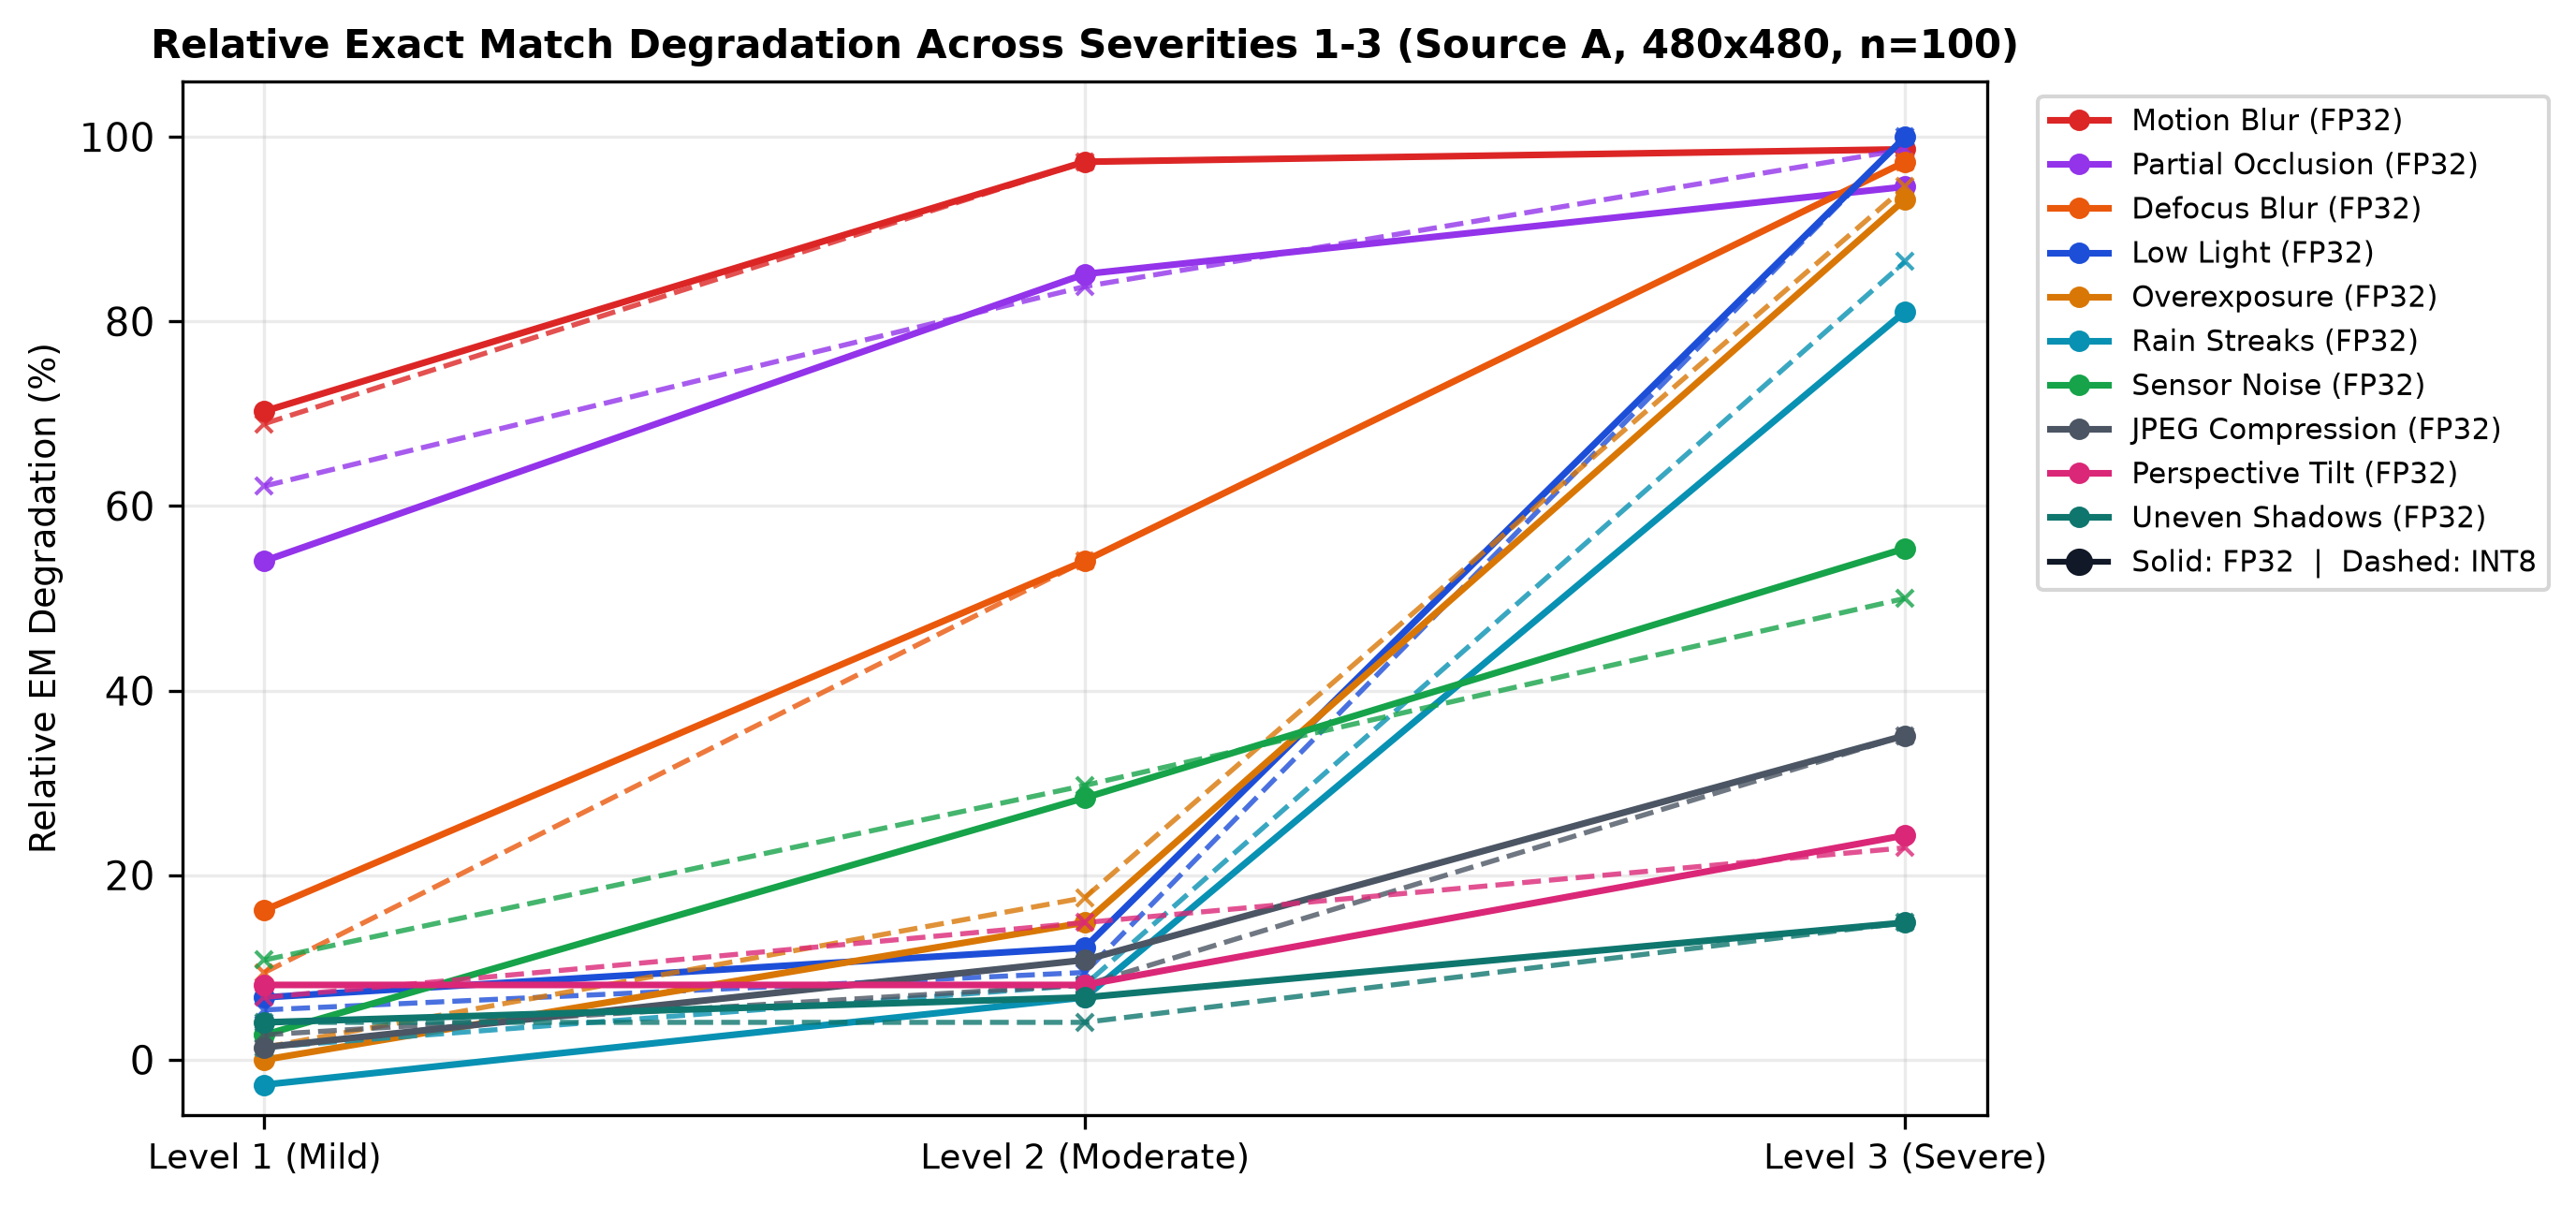
\includegraphics[width=0.95\textwidth]{figures/robustness_degradation.png}
    \caption{Relative Exact Match degradation (\%) across corruption severities 1--3 on the shared Source~A cohort ($480\times 480$).}\label{fig:degradation}
\end{figure}

\begin{figure}[t]
    \centering
    \begin{minipage}[b]{0.32\textwidth}
        \centering
        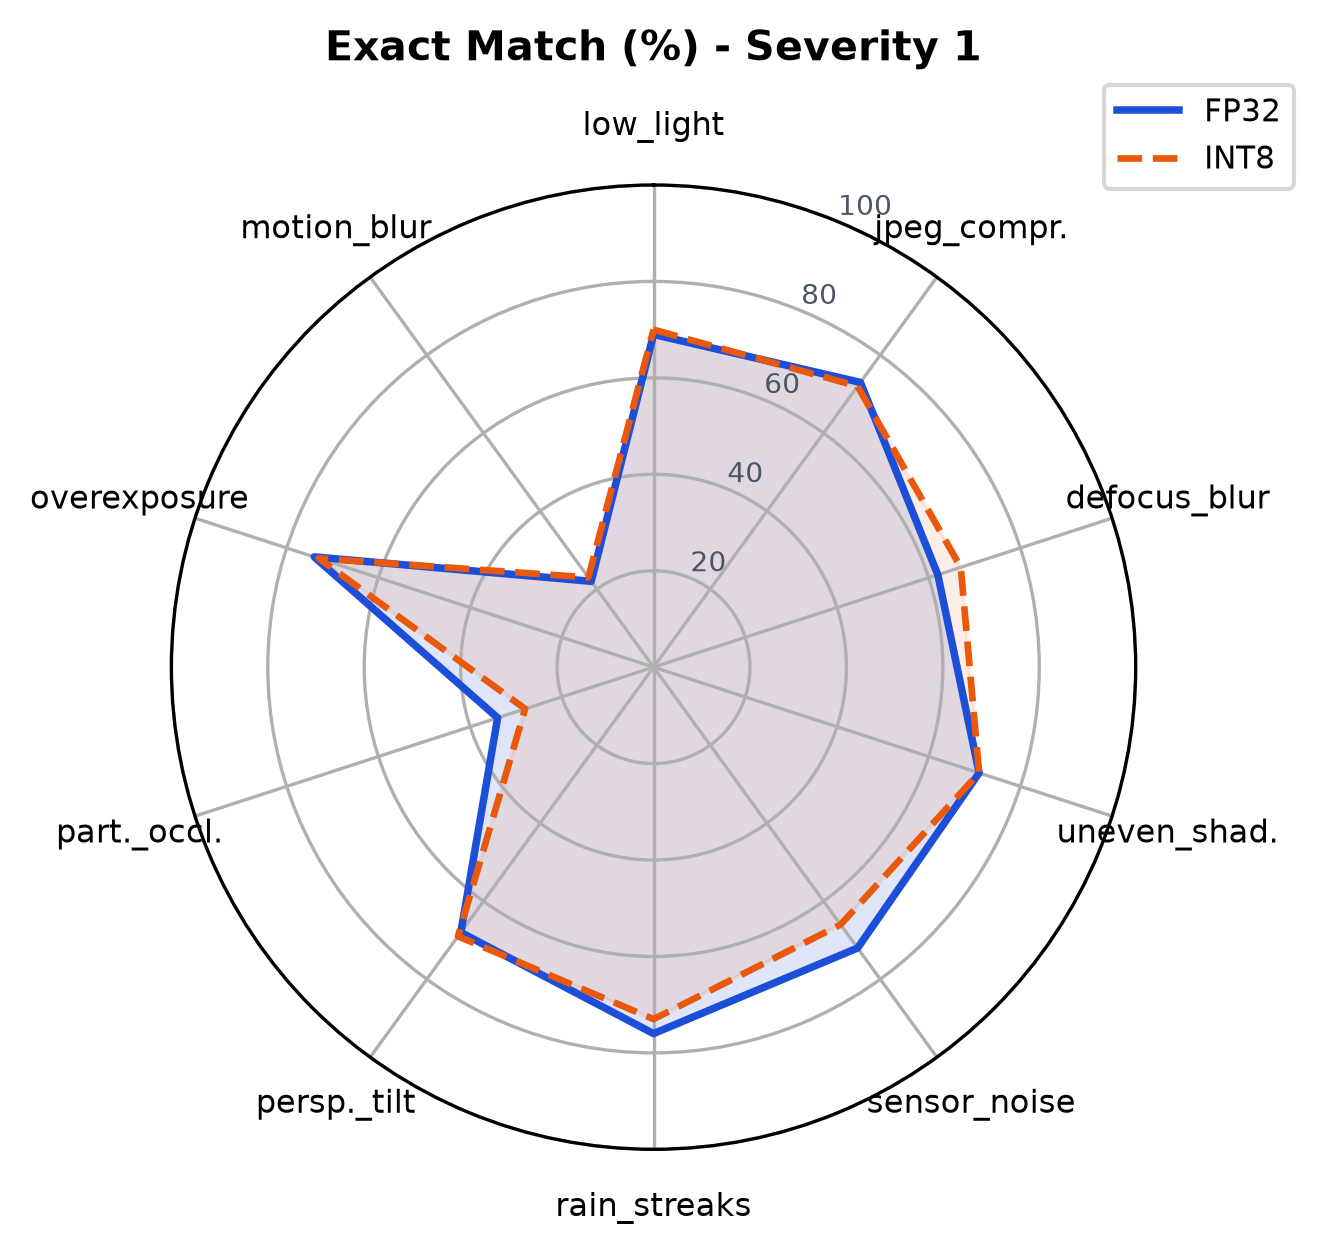
\includegraphics[width=\textwidth]{figures/radar_level1.png}
        \\[2pt]{\footnotesize (a) Level 1 (Mild)}
    \end{minipage}
    \hfill
    \begin{minipage}[b]{0.32\textwidth}
        \centering
        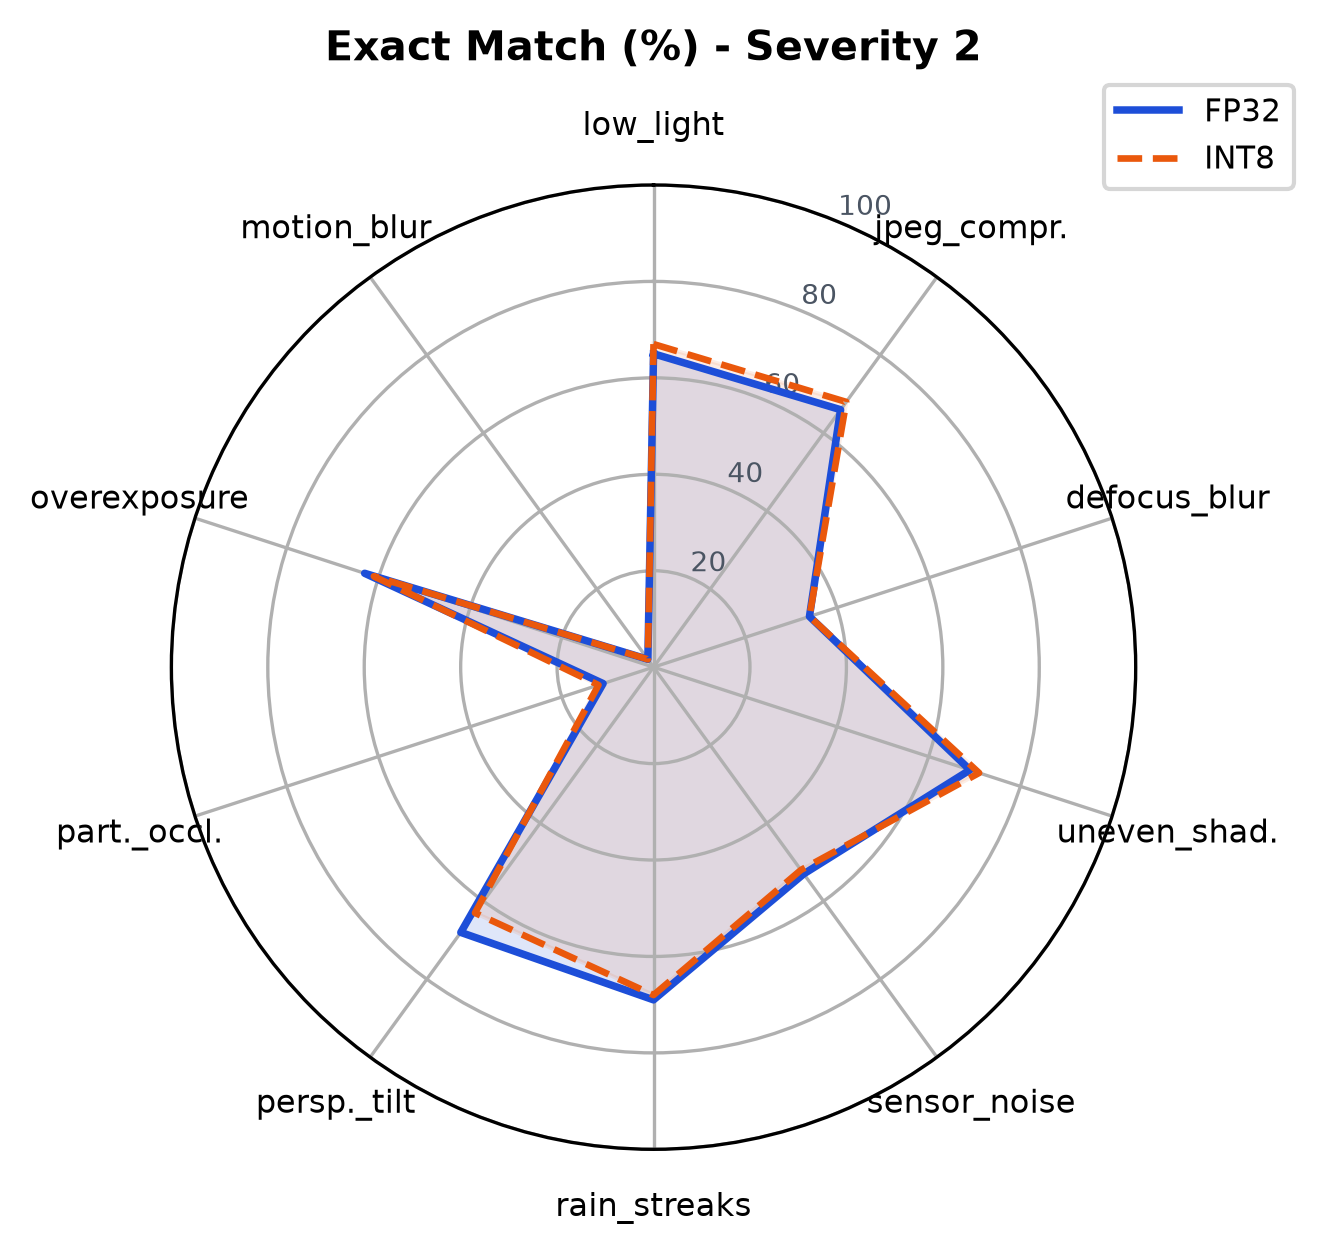
\includegraphics[width=\textwidth]{figures/radar_level2.png}
        \\[2pt]{\footnotesize (b) Level 2 (Moderate)}
    \end{minipage}
    \hfill
    \begin{minipage}[b]{0.32\textwidth}
        \centering
        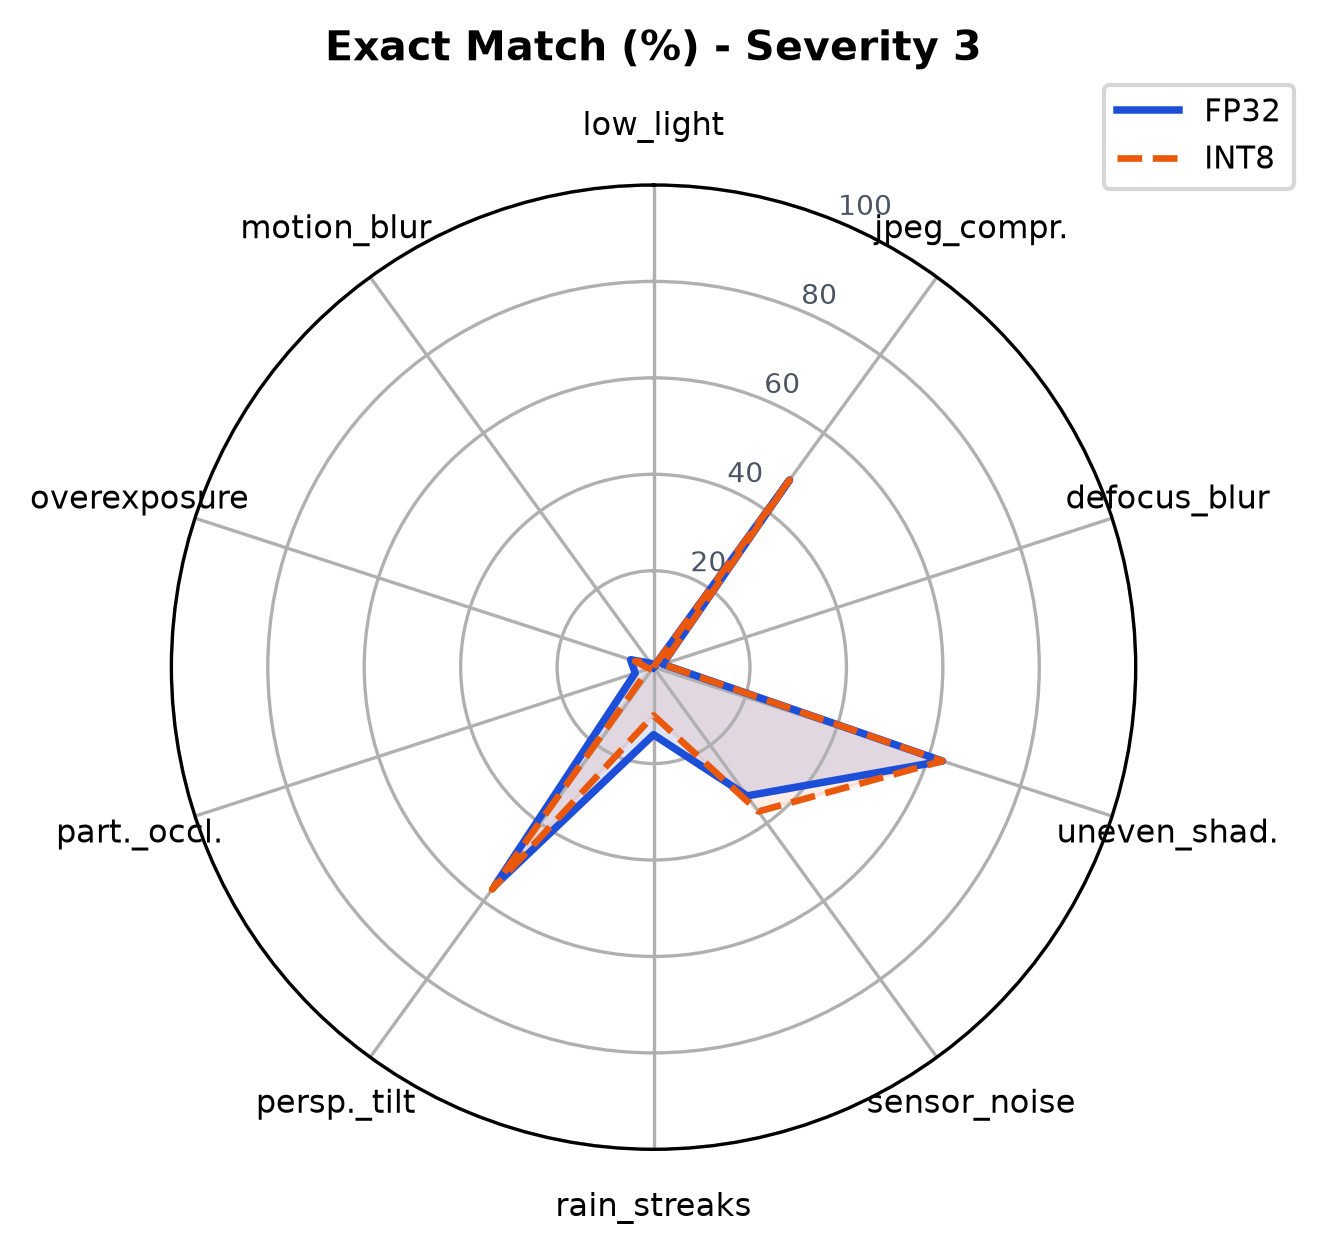
\includegraphics[width=\textwidth]{figures/radar_level3.png}
        \\[2pt]{\footnotesize (c) Level 3 (Severe)}
    \end{minipage}
    \caption{End-to-end Exact Match (\%) radar profiles comparing FP32 and INT8 across all 10 environmental perturbations at severity Levels 1, 2, and 3 ($480\times 480$, $N=100$).}\label{fig:radar}
\end{figure}

Three key conclusions emerge from Tables~\ref{tab:robustness_full}--\ref{tab:robustness_summary} and Figs.~\ref{fig:degradation}--\ref{fig:radar}:
\begin{enumerate}
    \item \textbf{Quantization preserves robustness:} Over 3,000 corrupted test evaluations per model, dynamic \texttt{QUInt8} compression tracks FP32 closely, with a mean signed deviation of only \textbf{$-0.09$\,pp} on mAP@50 and \textbf{$-0.47$\,pp} on EM (mean absolute EM difference $1.80$\,pp; maximum cell delta $\pm 6.00$\,pp, with INT8 outperforming FP32 on \texttt{defocus\_blur L1} by $+5.0$\,pp and \texttt{sensor\_noise L3} by $+4.0$\,pp).
    \item \textbf{Stage-wise decoupling between Detector and OCR resilience:} YOLOv8 maintains $>91\%$ mAP@50 even under severe \texttt{sensor\_noise-3} ($97.2\%$--$97.4\%$), \texttt{jpeg\_compression-3} ($98.2\%$--$98.6\%$), \texttt{partial\_occlusion-3} ($93.6\%$--$94.1\%$), and \texttt{motion\_blur-3} ($92.5\%$--$93.1\%$), breaking down only at extreme Level~3 optical losses (\texttt{overexposure-3}: $50.9\%$--$51.4\%$, \texttt{low\_light-3}: $56.6\%$--$59.8\%$, \texttt{rain\_streaks-3}: $66.3\%$--$66.8\%$). Conversely, RapidOCR collapses far earlier under \texttt{motion\_blur} (EM drops from $74.0\%$ to $22.0\%$--$23.0\%$ already at Level~1 despite $\sim 96\%$ mAP@50) and \texttt{partial\_occlusion} ($28.0\%$--$34.0\%$ at Level~1). Meanwhile, \texttt{uneven\_shadows-3} ($63.0\%$ EM) and \texttt{perspective\_tilt-3} ($56.0\%$--$57.0\%$ EM) remain comparatively tolerable.
    \item \textbf{Persistent 1-line vs.\ 2-line gap:} Across all 30 corrupted environments, one-line plates average $61.91\%$ EM (FP32) / $61.35\%$ EM (INT8)---more than double the accuracy on two-line plates ($29.81\%$ / $29.43\%$).
\end{enumerate}

\subsection{Real-World Sanity Check on Source B}\label{subsec:exp_sourceb}
Table~\ref{tab:source_b_slices} and Fig.~\ref{fig:source_b} dissect performance across the 4 real-world challenges of Source~B ($N=60$). Both models behave consistently across resolutions, with INT8 matching or slightly outperforming FP32 in detection across all four categories at $640$ and $480$. Critically, real-world EM ($28.3\%$--$38.3\%$) falls well below Source~A ($70.3\%$--$72.3\%$) due to two compounded factors: (i) 86.7\% of Source~B comprises stacked two-line plates, and (ii) the \emph{Geometry / Perspective Tilt} group consists 100\% (15/15) of steeply angled two-line motorcycle plates in cluttered backgrounds, yielding 6.67\%--13.33\% EM even when detector mAP@50 holds at 60.1\%--66.4\%. Similarly, physical headlight glare (\emph{High Glare}) induces blooming saturation that degrades $480\times 480$ mAP@50 to 32.0\%--35.4\% (intermediate between synthetic \texttt{overexposure} Levels 2 and 3). This contrast refutes overly optimistic weather accuracy claims (80.9\%--89.0\%) reported without strict End-to-End Exact Match or two-line separation in Paper~23~\cite{jagtap2025yolo}.

\begin{table}[t]
\centering
\caption{Source~B ($n=60$) slice evaluation across four physical field conditions (15 images/slice; metric pairs denote FP32/INT8 in \%).}\label{tab:source_b_slices}
{\fontsize{6.1pt}{7.4pt}\selectfont\setlength{\tabcolsep}{1.3pt}
\begin{tabular}{@{}>{\raggedright\arraybackslash}p{2.0cm}cccccccc@{}}
\toprule
 & & & \multicolumn{2}{c}{\textbf{640 (F/I \%)}} & \multicolumn{2}{c}{\textbf{480 (F/I \%)}} & \multicolumn{2}{c}{\textbf{320 (F/I \%)}} \\
\cmidrule(lr){4-5} \cmidrule(lr){6-7} \cmidrule(l){8-9}
\textbf{Slice ($n=15$)} & \textbf{2L} & \textbf{Bri./Shp.} & \textbf{mAP} & \textbf{EM} & \textbf{mAP} & \textbf{EM} & \textbf{mAP} & \textbf{EM} \\
\midrule
Low Light & 12/15 & 61.8/492.9 & 80.31/80.31 & 60.00/53.33 & 76.81/76.83 & 46.67/46.67 & 70.62/70.62 & 53.33/40.00 \\
Motion / Defocus Blur & 12/15 & 93.8/219.0 & 65.91/65.52 & 46.67/46.67 & 71.90/71.90 & 40.00/40.00 & 67.95/67.94 & 46.67/40.00 \\
High Glare / Overexp. & 13/15 & 145.6/399.9 & 48.55/\textbf{54.00} & 33.33/\textbf{40.00} & 32.01/35.43 & 26.67/20.00 & 42.34/43.70 & 33.33/33.33 \\
Geometry / Persp.\ Tilt & 15/15 & 102.0/780.8 & 60.05/\textbf{66.41} & 6.67/\textbf{13.33} & 65.30/66.37 & 6.67/6.67 & 42.01/46.81 & 6.67/13.33 \\
\midrule
\textbf{Overall (60)} & \textbf{52/60} & -- & 63.10/\textbf{65.95} & 36.67/\textbf{38.33} & 60.70/62.11 & 30.00/28.33 & 54.68/56.40 & 35.00/31.67 \\
\bottomrule
\end{tabular}%
}
\end{table}

\begin{figure}[t]
    \centering
    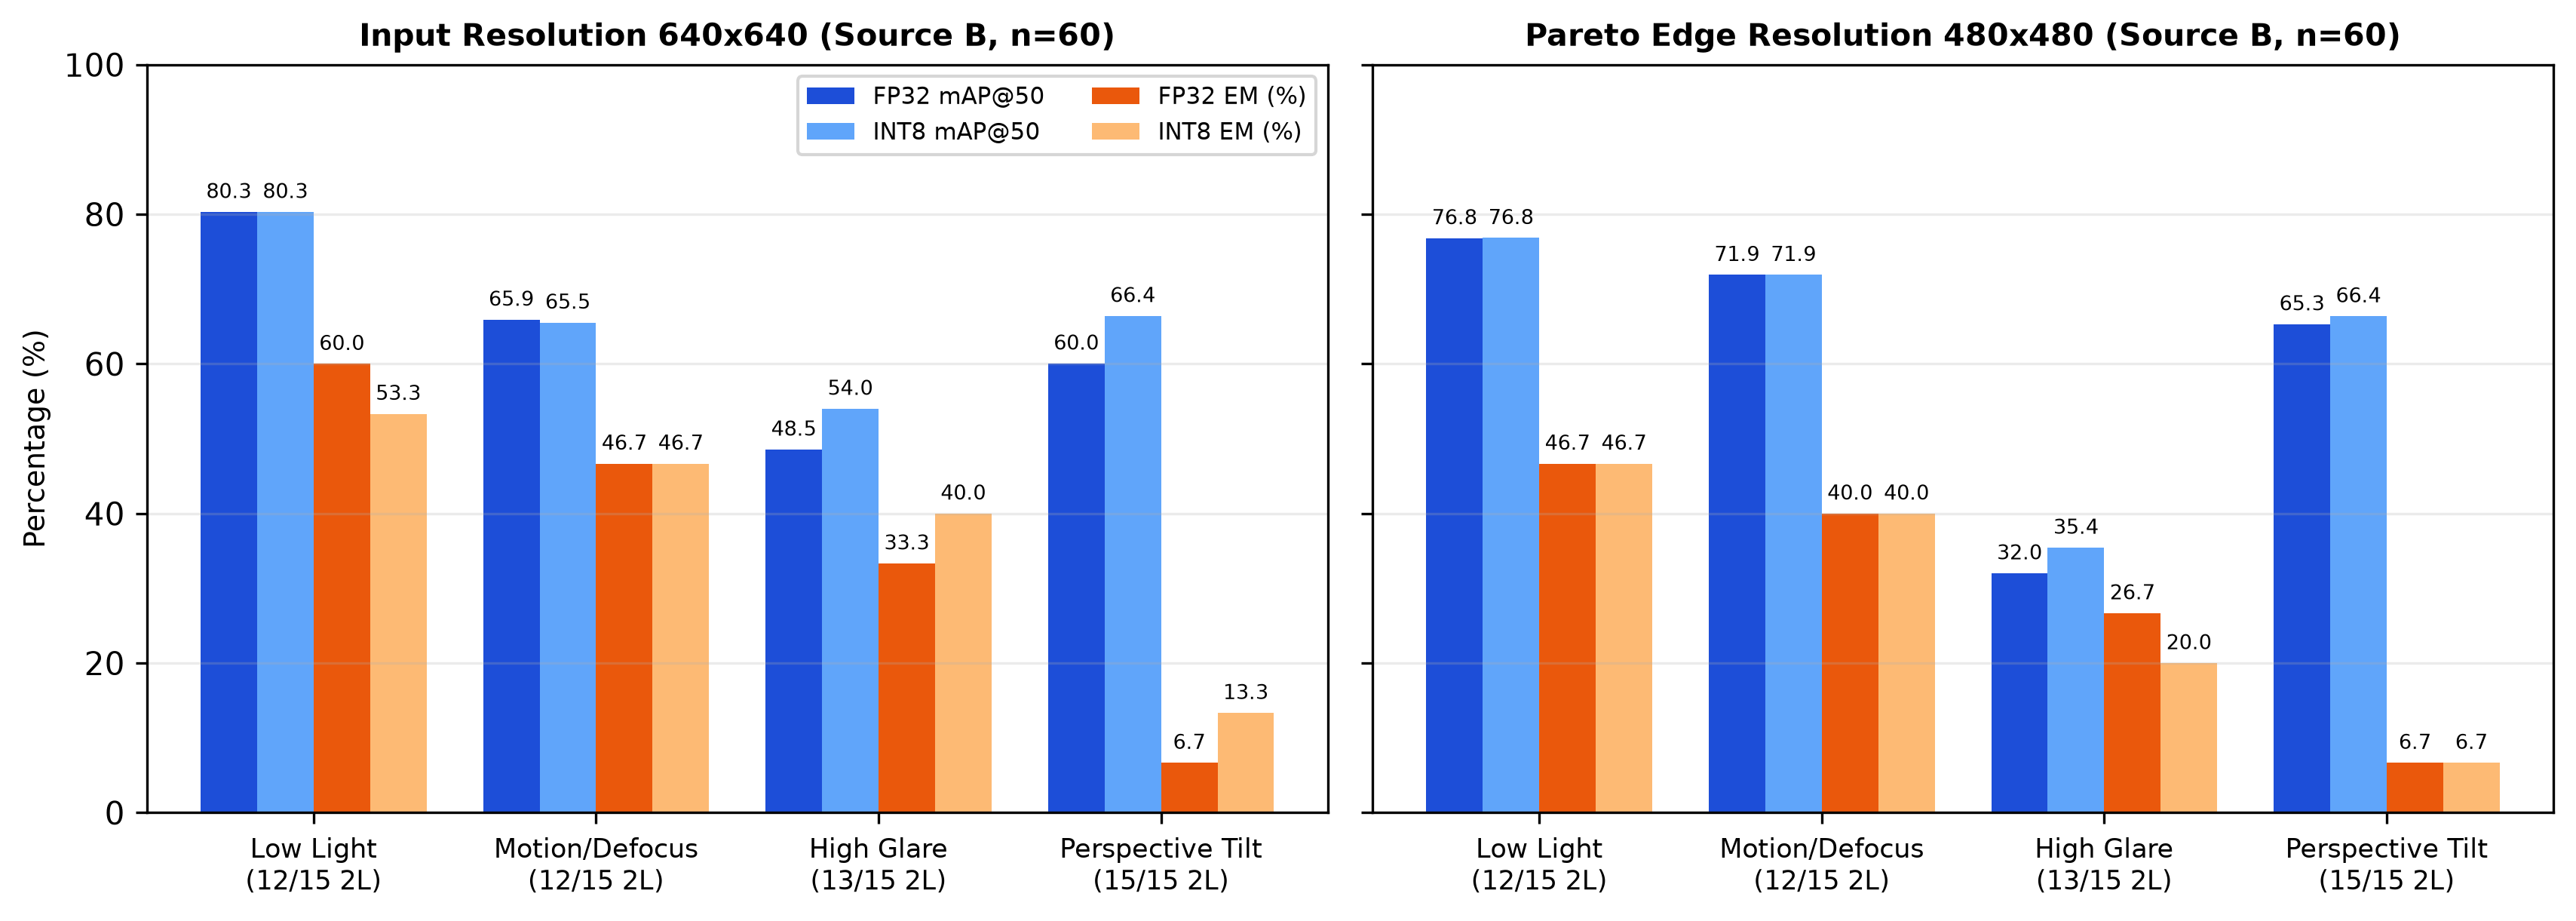
\includegraphics[width=\textwidth]{figures/source_b_slices.png}
    \caption{Source~B real-world slice comparison across four physical gate challenges at $640\times 640$ and Pareto $480\times 480$, demonstrating FP32/INT8 parity alongside severe two-line geometry and glare difficulty.}\label{fig:source_b}
\end{figure}

\subsection{Failure Mode Diagnosis and Threats to Validity}\label{subsec:failures}
Inspecting 3,840 failure records exported by \texttt{evaluation/error\_analysis.py} across all 64 robustness cells reveals three distinct failure mechanisms:
\begin{enumerate}
    \item \textbf{Optical Detector Collapse:} At \texttt{low\_light-3} and \texttt{overexposure-3}, edge contrast vanishes, generating 68 and 65 missed detections (INT8-$480$), respectively. Even the 32 plates detected under \texttt{low\_light-3} yield empty strings (e.g., GT \texttt{65B1-045.66} predicted as \texttt{""} at confidence 0.938) because cropped ROI luminance falls below DBNet's binarization threshold.
    \item \textbf{Early OCR Collapse Despite High-Confidence Detection:} Under \texttt{motion\_blur-1} (only 8 misses, 69 OCR mismatches for INT8) and \texttt{partial\_occlusion-1} (9 misses, 63 OCR mismatches), YOLOv8 retains $\sim 0.94$ confidence while character strokes smear or drop (e.g., \texttt{51G-222.37 $\rightarrow$ 51G-272.37}, \texttt{51G-436.30 $\rightarrow$ 51G-4360}). On clean two-line plates, DBNet frequently omits or merges upper-row series tokens (e.g., \texttt{94R1-9764 $\rightarrow$ 9764}, \texttt{63C1-3900 $\rightarrow$ 63C}).
    \item \textbf{Axis-Aligned Box Drift Under Extreme Perspective:} Under \texttt{perspective\_tilt-3} ($\approx 45^\circ$), axis-aligned ground-truth bounding boxes expand asymmetrically around slanted plates. Tighter detector predictions drop marginally below $\text{IoU}=0.50$, simultaneously generating 49 high-confidence ``false positives'' (up to confidence 0.945) and 26 missed detections even when $\Delta\text{IoU}$ on matched pairs stays 0.120.
\end{enumerate}

\textbf{Threats to Validity:} First, Source~A OCR text labels carry \texttt{labels\_verified=false} (\texttt{quality\_status="exploratory"}) because verified COCO geometry was paired with curated OCR annotations; absolute Source~A EM ceilings should therefore be interpreted relative to clean baseline deltas rather than human-audited ground truth. Second, while RPi hardware optimizations were measured under cgroup-limited Linux containers, the 64-cell robustness run executed on an \texttt{x86\_64} host CPU, where INT8 speedups do not manifest due to missing AVX-512 VNNI kernels. Third, sequential cell execution reuses Python allocator/OS caches, so observed RSS numbers denote process-level runtime observations rather than isolated per-cell cold boots.

\section{Conclusion and Future Work}\label{sec:conclusion}

This paper resolved critical efficiency, reproducibility, and evaluation blind spots in edge Vietnamese ALPR deployment. Replacing PyTorch with dynamic INT8 ONNX Runtime reduces initialization RAM by 83.8\% and weight files by over 71\% while surviving 256\,MB memory constraints. More importantly, diagnosing hidden OCR over-processing---eliminating RapidOCR's default 736\,px minimum-side upscaling via $H_{\max}=96$\,px ROI capping, \texttt{limit=320 max}, disabled dilation, and skipped angle classification alongside $480\times 480$ Pareto detector scaling and core-matched SIMD threads---accelerates OCR by $5.85\times$ and overall Raspberry Pi~4 pipeline speed by $6.26\times$ to 668.74\,ms. Finally, our transparent two-tier robustness evaluation across 9,000 synthetic corrupted variants and 60 adverse real-world captures confirms that INT8 quantization preserves robustness identically to FP32 ($\Delta\text{mAP@50}=-0.09$\,pp, $\Delta\text{EM}=-0.47$\,pp), while identifying OCR sensitivity to motion blur, partial occlusion, and skewed two-line motorcycle plates as top priorities for future research.

Future improvements will pursue: (i) lightweight ROI perspective rectification and adaptive local CLAHE preprocessing triggered selectively on low-luminance ROIs prior to DBNet; (ii) specialized CTC/attention recognizers trained natively on rectified two-line Vietnamese plates; (iii) full manual human audit of Source~A OCR ground truth; and (iv) on-device ARM64 verification directly on physical Raspberry Pi~4/5 hardware.

\backmatter

\bmhead{Acknowledgments}
The authors thank all members of the Embedded Computer Vision research team for collaborative engineering across dataset curation, synthetic perturbation generation, metric verification, benchmark orchestration, visualization, and Docker container packaging.

\section*{Declarations}
\begin{itemize}
    \item \textbf{Funding:} This research received no external funding.
    \item \textbf{Conflict of interest:} The authors declare no competing financial or non-financial interests.
    \item \textbf{Data and code availability:} Benchmark scripts, corruption generators, evaluation metrics, unit tests, and dataset manifests are maintained in the project repository (\url{https://github.com/HuyHo1405/260907_MSS301_Research}).
\end{itemize}

\bibliography{references}

\end{document}
